\chapter{Linear Algebra Basics: The Secret Language of AI}

% ============================================
% TikZ Style Definitions - Simple and Readable
% ============================================
\tikzset{
    % Axis styles - dark enough to read
    axis/.style={->, thick, black!60},
    axis label/.style={font=\footnotesize, black!70},
    % Grid styles
    grid/.style={very thin, black!15},
    % Vector styles - bold colors
    vec blue/.style={->, very thick, blue!80!black},
    vec red/.style={->, very thick, red!70!black},
    vec green/.style={->, very thick, green!50!black},
    vec purple/.style={->, very thick, purple!70!black},
    vec orange/.style={->, very thick, orange!70!black},
    % Label styles - simple and readable
    vec label/.style={font=\footnotesize},
    title label/.style={font=\footnotesize\bfseries},
    % Dashed helper lines
    helper/.style={dashed, black!40, thin},
}

\begin{center}
\textit{``Any sufficiently advanced technology is indistinguishable from magic.''} --- Arthur C. Clarke

\textit{``Any sufficiently analyzed magic is indistinguishable from linear algebra.''} --- This textbook
\end{center}

\section{The Day I Realized Words Are Just Lists of Numbers}

\textit{``Wait, you're telling me ChatGPT thinks in spreadsheets?''} — You, probably, in about 5 minutes.

Picture this: You're at a party (bear with me, this is going somewhere mathematical). Someone asks you to describe your friend Alex. You might say: ``Alex is funny, smart, kind of nerdy, loves coffee, hates mornings, super organized...''

Now imagine I'm an alien who doesn't understand human language. (Work with me here.) I need you to describe Alex in a way I can process. So you create a rating system:

\begin{center}
\begin{tabular}{lr}
\textbf{Trait} & \textbf{Rating (0-10)} \\
\hline
Funniness & 8 \\
Intelligence & 9 \\
Nerdiness & 7 \\
Coffee love & 10 \\
Morning person & 2 \\
Organization & 9 \\
\end{tabular}
\end{center}

Congratulations! You just created a \textbf{vector}: $\text{Alex} = [8, 9, 7, 10, 2, 9]$

\textit{This is literally how ChatGPT thinks about words.} I'm not kidding.

Every word---``cat,'' ``quantum,'' ``yesterday,'' ``love''---is a list of numbers, just like Alex. Except instead of 6 numbers, GPT-4 uses lists of \textit{12,288} numbers for each word. Twelve thousand! And all those mind-blowing things it does? Writing poetry? Explaining quantum physics? Helping debug your code at 2 AM? It's just math on these lists.

\textbf{Let that sink in:} The AI revolution is powered by adding and multiplying lists of numbers. That's it. That's the secret.

\begin{intuition}
\textbf{The Big Secret:} Linear algebra is the mathematics of lists (vectors) and tables (matrices) of numbers. That's it. That's the whole field.

If you can:
\begin{itemize}
    \item Add numbers \checkmark
    \item Multiply numbers \checkmark
\end{itemize}

Then you have everything you need to understand how AI thinks. I'm not dumbing this down---this is genuinely what's happening under the hood! The fancy terminology is just gift-wrapping.
\end{intuition}

\begin{connection}
\textbf{Why Should You Care About Linear Algebra?}

Here's the honest truth about modern AI:
\begin{itemize}
    \item \textbf{GPT-4, Claude, Gemini?} Linear algebra on steroids.
    \item \textbf{Image generators like DALL-E and Midjourney?} Linear algebra with extra steps.
    \item \textbf{Self-driving cars?} Linear algebra at 60 mph.
    \item \textbf{Recommendation algorithms (Netflix, Spotify, Amazon)?} Linear algebra deciding what you see.
\end{itemize}

If you want to understand how AI \textit{actually} works (not just use it, but understand it), linear algebra is your Rosetta Stone. And here's the beautiful part: it's not that hard! The core ideas are simple. The notation can look scary, but we'll demystify it together.

\textbf{By the end of this chapter, you'll be able to:}
\begin{enumerate}
    \item Understand what word embeddings actually are (and why they're magical)
    \item Read matrix equations without your eyes glazing over
    \item Explain to friends at parties why ``king - man + woman = queen'' works
    \item Feel genuinely comfortable with the math behind neural networks
\end{enumerate}

Let's go!
\end{connection}

\section{Vectors: Not as Scary as They Sound}

\subsection{What Even IS a Vector? (The Truth)}

Let me blow your mind with how simple this is. A \vocab{vector} is:
\begin{itemize}
    \item An ordered list of numbers
    \item That's it
    \item Seriously, that's the whole definition
    \item I'm not leaving anything out
\end{itemize}

\textbf{Two Ways to Think About Vectors:}

\textbf{1. As a list of numbers:} $[2, 3]$ means "the number 2, then the number 3"

\textbf{2. As an arrow:} An arrow that points from the origin to a location

\vspace{0.3cm}
\begin{center}
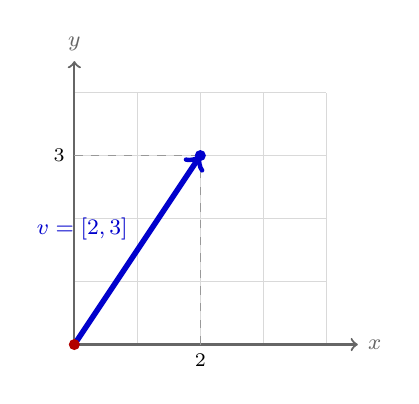
\begin{tikzpicture}[scale=0.8]
    % Grid
    \draw[grid] (0,0) grid (4,4);

    % Axes
    \draw[axis] (0,0) -- (4.5,0) node[right, font=\footnotesize] {$x$};
    \draw[axis] (0,0) -- (0,4.5) node[above, font=\footnotesize] {$y$};

    % Helper lines (dashed projections)
    \draw[helper] (2,0) -- (2,3);
    \draw[helper] (0,3) -- (2,3);

    % The vector
    \draw[vec blue, line width=2pt] (0,0) -- (2,3);

    % Vector label
    \node[blue!80!black, font=\footnotesize, above left] at (1,1.5) {$\vect{v} = [2,3]$};

    % Endpoint and origin markers
    \fill[blue!80!black] (2,3) circle (2.5pt);
    \fill[red!70!black] (0,0) circle (2.5pt);

    % Component labels
    \node[below, font=\scriptsize] at (2,0) {2};
    \node[left, font=\scriptsize] at (0,3) {3};
\end{tikzpicture}
\end{center}
\vspace{0.3cm}

\textbf{Think of it like giving directions:} ``Go 2 blocks east, then 3 blocks north.'' That's the vector $[2, 3]$! You've been doing linear algebra every time you used Google Maps. Congratulations, you're already a mathematician.

Here's the notation mathematicians use (don't let it intimidate you):

\begin{example}
\textbf{These are all vectors:}
\[
\vect{v} = \begin{bmatrix} 2 \\ 3 \end{bmatrix} \quad \text{(your GPS location: 2 km east, 3 km north)}
\]
\[
\vect{w} = \begin{bmatrix} 255 \\ 140 \\ 0 \end{bmatrix} \quad \text{(an orange color: red=255, green=140, blue=0)}
\]
\[
\vect{recipe} = \begin{bmatrix} 2 \\ 3 \\ 0.5 \\ 1 \end{bmatrix} \quad \text{(2 eggs, 3 cups flour, 0.5 tsp salt, 1 cup sugar)}
\]

We say $\vect{v}$ is "2-dimensional" (2 numbers), $\vect{w}$ is "3-dimensional" (3 numbers), and $\vect{recipe}$ is "4-dimensional" (4 numbers).
\end{example}

\textbf{The fancy math notation:} When you see $\vect{v} \in \R^2$, it just means "v is a list of 2 real numbers." The $\R$ stands for "real numbers" (as opposed to imaginary numbers, but don't worry about those). The superscript 2 is how many numbers are in the list.

\textbf{"But I thought vectors were arrows!"}

Great question! They ARE arrows (in 2D and 3D)! Here's the beautiful part: a list of numbers AND an arrow are the SAME thing, just viewed differently.

\begin{center}
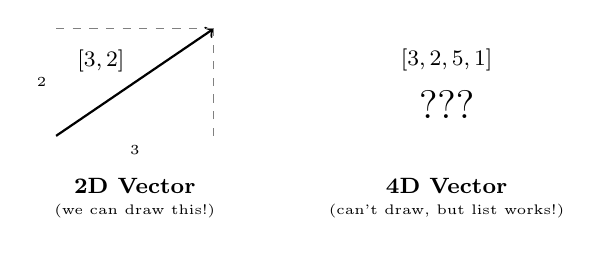
\begin{tikzpicture}[scale=0.8]
    % 2D vector (left side)
    \begin{scope}
    \draw[->,thick] (0,0) -- (2.5,1.7) node[midway,above left] {\footnotesize $[3, 2]$};
    \draw[dashed,gray] (2.5,0) -- (2.5,1.7);
    \draw[dashed,gray] (0,1.7) -- (2.5,1.7);
    \node[below] at (1.25,0) {\tiny 3};
    \node[left] at (0,0.85) {\tiny 2};
    \node at (1.25,-0.8) {\footnotesize \textbf{2D Vector}};
    \node at (1.25,-1.2) {\tiny (we can draw this!)};
    \end{scope}

    % 4D vector (right side)
    \begin{scope}[xshift=5cm]
    \node at (1.2,1.2) {\footnotesize $[3, 2, 5, 1]$};
    \node at (1.2,0.5) {\Large ???};
    \node at (1.2,-0.8) {\footnotesize \textbf{4D Vector}};
    \node at (1.2,-1.2) {\tiny (can't draw, but list works!)};
    \end{scope}
\end{tikzpicture}
\end{center}

When you have a vector with 12,288 dimensions (like in GPT-4), you \textit{definitely} can't draw that arrow. Our brains max out at 3D, and even that's pushing it. But the list of numbers works perfectly in any dimension! The arrow is a helpful picture for 2D/3D, but the list is the universal definition that works everywhere.

\textbf{Fun fact:} Mathematicians in the 1800s got into heated arguments about whether ``4D vectors'' were even a real thing. William Rowan Hamilton literally carved his breakthrough equation into a bridge in Dublin because he was so excited about 4D numbers. Now we casually use 12,000-dimensional vectors to generate cat pictures. Times change!

\textbf{A note on notation:} You'll see vectors written in different ways:
\begin{itemize}
    \item $\vect{v}$ or $\mathbf{v}$ (bold letter)---common in textbooks
    \item $\vec{v}$ (arrow on top)---common in physics
    \item $[1, 2, 3]$ (list/array notation)---common in programming
    \item $\begin{bmatrix} 1 \\ 2 \\ 3 \end{bmatrix}$ (column vector)---common in math
\end{itemize}
They all mean the same thing! Different fields have different preferences. We'll mostly use bold letters and column vectors.

\textbf{Bottom line:} In 2D/3D, use whichever mental model helps you. For higher dimensions, stick with "list of numbers."

\begin{connection}
\textbf{How ChatGPT uses vectors:}

Every word in ChatGPT's vocabulary is a vector with thousands of dimensions. The word "king" might look like:
\[
\text{``king''} = \begin{bmatrix} 0.23 \\ -0.45 \\ 0.89 \\ 0.12 \\ \vdots \\ -0.34 \end{bmatrix} \in \R^{12288}
\]

That's 12,288 numbers! Each dimension captures some abstract aspect of "kingness." Maybe:
\begin{itemize}
    \item Dimension 47 represents "royalty"
    \item Dimension 892 represents "male-associated concepts"
    \item Dimension 3,421 represents "power/authority"
\end{itemize}

The crazy part? The AI figures out what each dimension means \textit{on its own} just by reading tons of text. Nobody programs in "dimension 47 = royalty." It just... emerges. (Mind = blown, right?)
\end{connection}

\subsection{Vector Addition: Combining Personalities (and Arrows!)}

Now for the fun part—what can we DO with vectors?

\textbf{The Personality Blend:}

Let's say you have two friends:
\begin{itemize}
    \item Sarah = [Funny: 9, Athletic: 8, Bookish: 3]
    \item Morgan = [Funny: 4, Athletic: 3, Bookish: 10]
\end{itemize}

What if you wanted to describe a person who's kind of a blend of both? You'd add them!

\[
\text{Sarah + Morgan} = \begin{bmatrix} 9 \\ 8 \\ 3 \end{bmatrix} + \begin{bmatrix} 4 \\ 3 \\ 10 \end{bmatrix} = \begin{bmatrix} 9+4 \\ 8+3 \\ 3+10 \end{bmatrix} = \begin{bmatrix} 13 \\ 11 \\ 13 \end{bmatrix}
\]

This new person would be super funny (13), quite athletic (11), and very bookish (13)—a blend of both personalities!

\textbf{The Geometric View (This is Beautiful!):}

When you add vectors as arrows, you place them \textit{tip-to-tail}:

\vspace{0.3cm}
\begin{center}
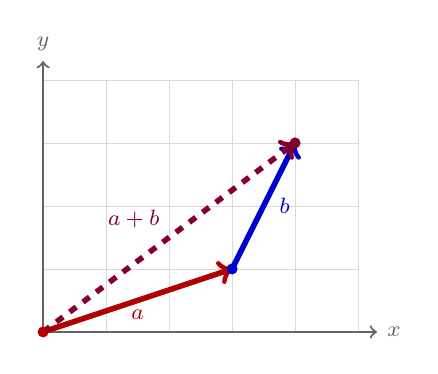
\begin{tikzpicture}[scale=0.8]
    % Grid
    \draw[grid] (0,0) grid (5,4);

    % Axes
    \draw[axis] (0,0) -- (5.3,0) node[right, font=\footnotesize] {$x$};
    \draw[axis] (0,0) -- (0,4.3) node[above, font=\footnotesize] {$y$};

    % First vector (red)
    \draw[vec red, line width=2pt] (0,0) -- (3,1);
    \node[red!70!black, font=\footnotesize, below] at (1.5,0.5) {$\vect{a}$};

    % Second vector (blue)
    \draw[vec blue, line width=2pt] (3,1) -- (4,3);
    \node[blue!80!black, font=\footnotesize, right] at (3.6,2) {$\vect{b}$};

    % Result vector (purple, dashed)
    \draw[vec purple, line width=2pt, dashed] (0,0) -- (4,3);
    \node[purple!70!black, font=\footnotesize, above left] at (2,1.5) {$\vect{a}+\vect{b}$};

    % Points
    \fill[red!70!black] (0,0) circle (2.5pt);
    \fill[blue!80!black] (3,1) circle (2.5pt);
    \fill[purple!70!black] (4,3) circle (2.5pt);
\end{tikzpicture}
\end{center}
\vspace{0.2cm}
\textit{Walk $\vect{a}$, then walk $\vect{b}$. The purple arrow is your total journey!}
\vspace{0.3cm}

\textbf{Think of it like walking:} Walk 3 blocks east and 1 north (red arrow). Then from there, walk 1 more east and 2 north (blue arrow). Where do you end up? 4 blocks east and 3 north (purple arrow)! That's vector addition!

\begin{definition}{Vector Addition}{}
To add two vectors, just add their corresponding components (the numbers in the same positions):
\[
\vect{a} + \vect{b} = \begin{bmatrix} a_1 \\ a_2 \\ \vdots \\ a_n \end{bmatrix} + \begin{bmatrix} b_1 \\ b_2 \\ \vdots \\ b_n \end{bmatrix} = \begin{bmatrix} a_1 + b_1 \\ a_2 + b_2 \\ \vdots \\ a_n + b_n \end{bmatrix}
\]

\textbf{Important:} You can only add vectors that have the same number of dimensions. You can't add [1, 2] and [3, 4, 5]—that's like trying to add apples and a spaceship.
\end{definition}

\begin{example}
Let's add some recipe vectors (why not?):
\[
\begin{bmatrix} 2 \text{ eggs} \\ 3 \text{ cups flour} \\ 1 \text{ cup sugar} \end{bmatrix} + \begin{bmatrix} 3 \text{ eggs} \\ 1 \text{ cup flour} \\ 2 \text{ cups sugar} \end{bmatrix} = \begin{bmatrix} 5 \text{ eggs} \\ 4 \text{ cups flour} \\ 3 \text{ cups sugar} \end{bmatrix}
\]

You just combined two recipes into one mega-recipe! (Whether it tastes good is... another question.)
\end{example}

\begin{intuition}
\textbf{Multiple ways to understand vector addition:}

\textbf{As lists:} Add each number separately: $[3,1] + [1,2] = [3+1, 1+2] = [4,3]$

\textbf{As arrows:} Place them tip-to-tail and draw the direct path from start to finish

\textbf{As movement:} First move, then second move = total movement

\textbf{As ingredients:} Combining recipes, mixing paint colors, blending personalities

\textbf{Fun fact:} Order doesn't matter! $\vect{a} + \vect{b} = \vect{b} + \vect{a}$ (just like $3 + 5 = 5 + 3$)

\vspace{0.3cm}
\begin{center}
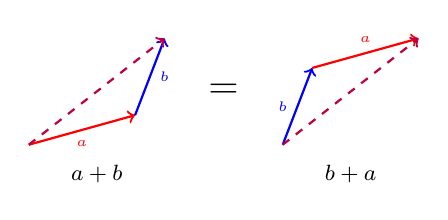
\begin{tikzpicture}[scale=0.75]
    % Left: a then b
    \begin{scope}
    \draw[->,thick,red] (0,0) -- (1.8,0.5) node[midway,below] {\tiny $\vect{a}$};
    \draw[->,thick,blue] (1.8,0.5) -- (2.3,1.8) node[midway,right] {\tiny $\vect{b}$};
    \draw[->,thick,purple,dashed] (0,0) -- (2.3,1.8);
    \node at (1.15,-0.5) {\footnotesize $\vect{a} + \vect{b}$};
    \end{scope}

    % Equals sign
    \node at (3.3,0.9) {\Large $=$};

    % Right: b then a
    \begin{scope}[xshift=4.3cm]
    \draw[->,thick,blue] (0,0) -- (0.5,1.3) node[midway,left] {\tiny $\vect{b}$};
    \draw[->,thick,red] (0.5,1.3) -- (2.3,1.8) node[midway,above] {\tiny $\vect{a}$};
    \draw[->,thick,purple,dashed] (0,0) -- (2.3,1.8);
    \node at (1.15,-0.5) {\footnotesize $\vect{b} + \vect{a}$};
    \end{scope}
\end{tikzpicture}

\textit{Same destination! Order doesn't matter! (Mathematicians call this ``commutative.'')}
\end{center}
\vspace{0.3cm}
\end{intuition}

\begin{connection}
\textbf{In transformers (the AI architecture):}

When processing the sentence "The cat sat on the mat," the model needs to combine information from different words. It literally adds their vector representations together!

For example, to understand "cat," the model might add:
\begin{itemize}
    \item The meaning of "cat" itself
    \item Context from "The" (it's a specific cat)
    \item Spatial info from "sat on the mat"
\end{itemize}

All of this is vector addition happening thousands of times per second!
\end{connection}

\subsection{Scalar Multiplication: Turning the Volume Up or Down}

What if you want to make something \textit{more intense}? That's scalar multiplication.

\textbf{Quick vocab:} "Scalar" is just a fancy word for "regular number" (like 2, 3.5, or -1). When you multiply a vector by a scalar, you're stretching or shrinking it:

\vspace{0.3cm}
\begin{center}
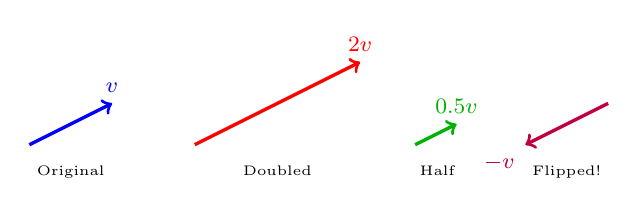
\begin{tikzpicture}[scale=0.7]
    % Top row: Original and Doubled
    \begin{scope}
    \draw[->,very thick,blue] (0,0) -- (1.5,0.75) node[above] {\footnotesize $\vect{v}$};
    \node[below] at (0.75,-0.2) {\tiny Original};
    \end{scope}

    \begin{scope}[xshift=3cm]
    \draw[->,very thick,red] (0,0) -- (3,1.5) node[above] {\footnotesize $2\vect{v}$};
    \node[below] at (1.5,-0.2) {\tiny Doubled};
    \end{scope}

    % Bottom row: Half and Flipped
    \begin{scope}[xshift=7cm]
    \draw[->,very thick,green!70!black] (0,0) -- (0.75,0.375) node[above] {\footnotesize $0.5\vect{v}$};
    \node[below] at (0.4,-0.2) {\tiny Half};
    \end{scope}

    \begin{scope}[xshift=9cm]
    \draw[->,very thick,purple] (1.5,0.75) -- (0,0) node[below left] {\footnotesize $-\vect{v}$};
    \node[below] at (0.75,-0.2) {\tiny Flipped!};
    \end{scope}
\end{tikzpicture}
\end{center}
\vspace{0.3cm}

\textbf{What's happening:}
\begin{itemize}
    \item Multiply by 2: Arrow becomes twice as long (same direction)
    \item Multiply by 0.5: Arrow becomes half as long (same direction)
    \item Multiply by -1: Arrow flips to opposite direction!
    \item Multiply by 0: Arrow shrinks to nothing (just a dot at origin)
\end{itemize}

\begin{definition}{Scalar Multiplication}{}
Multiply every component of the vector by the scalar:
\[
c \cdot \vect{v} = c \cdot \begin{bmatrix} v_1 \\ v_2 \\ \vdots \\ v_n \end{bmatrix} = \begin{bmatrix} c \cdot v_1 \\ c \cdot v_2 \\ \vdots \\ c \cdot v_n \end{bmatrix}
\]

\textbf{Special cases that will come up a lot:}
\begin{itemize}
    \item $1 \cdot \vect{v} = \vect{v}$ (identity---nothing changes)
    \item $0 \cdot \vect{v} = \vect{0}$ (annihilation---everything becomes zero)
    \item $(-1) \cdot \vect{v} = -\vect{v}$ (negation---flip the direction)
\end{itemize}
\end{definition}

\begin{example}
Remember our friend Alex? $\text{Alex} = [8, 9, 7, 10, 2, 9]$ (funny, smart, nerdy, coffee-loving, NOT a morning person, organized)

What if we meet Alex \textit{after 3 cups of espresso}? Everything gets amplified!
\[
3 \times \text{Alex} = 3 \times \begin{bmatrix} 8 \\ 9 \\ 7 \\ 10 \\ 2 \\ 9 \end{bmatrix} = \begin{bmatrix} 24 \\ 27 \\ 21 \\ 30 \\ 6 \\ 27 \end{bmatrix}
\]

Super funny (24), ultra smart (27), mega organized (27), and even slightly tolerable in the morning (6)!

What about $0.5 \times \text{Alex}$? That's Alex on Monday morning before coffee:
\[
0.5 \times \text{Alex} = \begin{bmatrix} 4 \\ 4.5 \\ 3.5 \\ 5 \\ 1 \\ 4.5 \end{bmatrix}
\]

Half the energy, half the enthusiasm. Morning person score dropped to 1. We've all been there. Some of us are writing math textbooks in that state right now.
\end{example}

\begin{intuition}
\textbf{Think of scalar multiplication like a volume knob or zoom button:}

\begin{itemize}
    \item \textbf{Scalar > 1:} ZOOM IN! Make it bigger! "Turn up the volume!"
    \item \textbf{Scalar = 1:} No change (like multiplying by 1 in regular math)
    \item \textbf{0 < Scalar < 1:} Zoom out, make it smaller
    \item \textbf{Scalar = 0:} Mute! Vector disappears to $[0,0]$
    \item \textbf{Scalar < 0:} Reverse direction! Like rewinding
\end{itemize}

\textbf{Real-world examples:}
\begin{itemize}
    \item Recipe for 4 people? Multiply recipe vector by 4!
    \item Want to go backwards? Multiply movement vector by -1!
    \item Zooming in on a map? Multiply coordinate vectors by zoom factor!
\end{itemize}

\textbf{The key insight:} Direction stays the same (unless you use a negative scalar), only the length changes!
\end{intuition}

\begin{connection}
\textbf{In neural networks:}

Every connection between neurons has a "weight" (a scalar). The signal gets multiplied by this weight as it travels. A weight of 2.0 means "this is important, amplify it!" A weight of 0.1 means "this barely matters." A weight of -1.5 means "this is important but in the opposite way, inhibit it!"

This is how neural networks learn—by adjusting millions of these scalar multipliers until the network does what we want.
\end{connection}

\begin{intuition}
\textbf{The Emotion Dial Analogy}

Imagine your personality vector: [Happiness, Anxiety, Excitement, Tiredness]

\textbf{Monday morning:} $0.3 \times \text{You} = [0.3 \times \text{Happy}, 0.3 \times \text{Anxious}, ...]$

Everything is muted. You're operating at 30\% capacity.

\textbf{Friday evening:} $1.5 \times \text{You}$

Everything is amplified! More happy, but also if you were anxious, more anxious.

\textbf{Key insight:} Scalar multiplication changes the \textit{intensity} but not the \textit{character}. A scared person scaled by 2 becomes a very scared person, not a happy person. The ratios between components stay the same!

This is crucial in ML: when we normalize vectors (scale them to length 1), we're removing intensity and keeping only the ``direction''---the character of the information.
\end{intuition}

\subsection{The Dot Product: The Most Important Thing You'll Learn Today}

Okay, this is where it gets REALLY exciting. The \vocab{dot product} (also called \vocab{inner product}) is the secret sauce of machine learning. It measures how much two vectors "agree" with each other.

\textbf{Before we dive into the formula, let's build intuition...}

Imagine two arrows pointing in space. Ask yourself: "Are they pointing in similar directions or opposite directions?"

\vspace{0.3cm}
\begin{center}
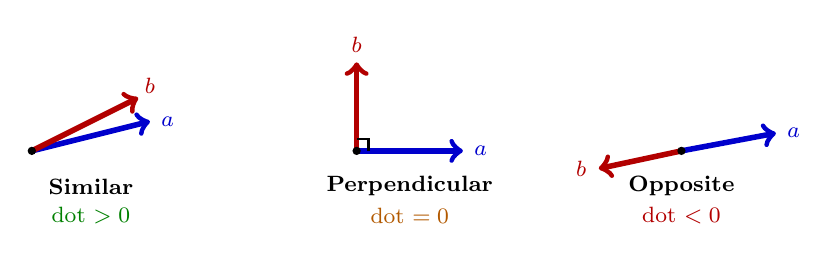
\begin{tikzpicture}[scale=0.75]
    % Similar directions (left)
    \begin{scope}
        \draw[vec blue, line width=2pt] (0,0) -- (2,0.5);
        \draw[vec red, line width=2pt] (0,0) -- (1.8,0.9);
        \node[blue!80!black, font=\footnotesize] at (2.3,0.5) {$\vect{a}$};
        \node[red!70!black, font=\footnotesize] at (2,1.1) {$\vect{b}$};
        \fill[black] (0,0) circle (2pt);
        \node[font=\footnotesize\bfseries] at (1,-0.6) {Similar};
        \node[font=\footnotesize, green!50!black] at (1,-1.1) {dot $> 0$};
    \end{scope}

    % Perpendicular (middle)
    \begin{scope}[xshift=5.5cm]
        \draw[vec blue, line width=2pt] (0,0) -- (1.8,0);
        \draw[vec red, line width=2pt] (0,0) -- (0,1.5);
        \node[blue!80!black, font=\footnotesize] at (2.1,0) {$\vect{a}$};
        \node[red!70!black, font=\footnotesize] at (0,1.8) {$\vect{b}$};
        \draw[black, thick] (0.2,0) -- (0.2,0.2) -- (0,0.2);
        \fill[black] (0,0) circle (2pt);
        \node[font=\footnotesize\bfseries] at (0.9,-0.6) {Perpendicular};
        \node[font=\footnotesize, orange!70!black] at (0.9,-1.1) {dot $= 0$};
    \end{scope}

    % Opposite (right)
    \begin{scope}[xshift=11cm]
        \draw[vec blue, line width=2pt] (0,0) -- (1.6,0.3);
        \draw[vec red, line width=2pt] (0,0) -- (-1.4,-0.3);
        \node[blue!80!black, font=\footnotesize] at (1.9,0.3) {$\vect{a}$};
        \node[red!70!black, font=\footnotesize] at (-1.7,-0.3) {$\vect{b}$};
        \fill[black] (0,0) circle (2pt);
        \node[font=\footnotesize\bfseries] at (0,-0.6) {Opposite};
        \node[font=\footnotesize, red!70!black] at (0,-1.1) {dot $< 0$};
    \end{scope}
\end{tikzpicture}
\end{center}
\vspace{0.3cm}

\textbf{The dot product is a SINGLE NUMBER that tells you:} "How much do these vectors point in the same direction?"

\begin{definition}{Dot Product}{}
To compute the dot product of two vectors, multiply corresponding components and add up the results:
\[
\vect{a} \cdot \vect{b} = a_1 b_1 + a_2 b_2 + \cdots + a_n b_n = \sum_{i=1}^{n} a_i b_i
\]

It takes two vectors as input and gives you a single number as output.
\end{definition}

\begin{intuition}
\textbf{The "Agreement Score" Interpretation}

Think of the dot product as a compatibility quiz between two vectors. For each dimension:
\begin{itemize}
    \item If both numbers are positive (they agree), you add a positive contribution
    \item If both are negative (they agree on the negative side), you ALSO add positive (negative times negative)
    \item If one is positive and one is negative (they disagree), you add negative
    \item If either is zero (one doesn't care), no contribution
\end{itemize}

The final number is the total "agreement score"!

\textbf{Analogy: The Blind Date Algorithm}

Imagine a dating app that rates people on various traits from -10 to +10:
\begin{center}
\begin{tabular}{lccc}
\textbf{Trait} & \textbf{You} & \textbf{Date A} & \textbf{Date B} \\
\hline
Loves outdoors & +8 & +9 & -7 \\
Night owl & -5 & -6 & +8 \\
Likes spicy food & +7 & +3 & +2 \\
\end{tabular}
\end{center}

Dot product with Date A: $(8)(9) + (-5)(-6) + (7)(3) = 72 + 30 + 21 = 123$ (Great match!)

Dot product with Date B: $(8)(-7) + (-5)(8) + (7)(2) = -56 - 40 + 14 = -82$ (Disaster!)

The math literally quantifies compatibility!
\end{intuition}

\begin{example}
Let's compute a dot product:
\[
\begin{bmatrix} 1 \\ 2 \\ 3 \end{bmatrix} \cdot \begin{bmatrix} 4 \\ -1 \\ 2 \end{bmatrix} = (1 \times 4) + (2 \times -1) + (3 \times 2) = 4 - 2 + 6 = 8
\]

Another one:
\[
\begin{bmatrix} 2 \\ 3 \end{bmatrix} \cdot \begin{bmatrix} 5 \\ 7 \end{bmatrix} = (2 \times 5) + (3 \times 7) = 10 + 21 = 31
\]
\end{example}

\textbf{"Okay, but WHY does this matter?"}

Great question! The dot product tells you how \textit{similar} two vectors are:

\begin{itemize}
    \item \textbf{Large positive:} Vectors point in similar directions
    \item \textbf{Near zero:} Vectors are perpendicular/unrelated
    \item \textbf{Large negative:} Vectors point in opposite directions
\end{itemize}

\begin{example}
\textbf{Movie preferences:}

You rate movies as [Action, Romance, Comedy, Horror]:
\begin{itemize}
    \item You: [9, 2, 8, 1] (love action and comedy, not into romance or horror)
    \item Friend A: [8, 3, 9, 0] (similar taste!)
    \item Friend B: [1, 10, 2, 9] (loves romance and horror, hates action)
\end{itemize}

Dot products:
\[
\text{You} \cdot \text{Friend A} = (9)(8) + (2)(3) + (8)(9) + (1)(0) = 72 + 6 + 72 + 0 = 150
\]
\[
\text{You} \cdot \text{Friend B} = (9)(1) + (2)(10) + (8)(2) + (1)(9) = 9 + 20 + 16 + 9 = 54
\]

Friend A has a much higher dot product with you (150 vs 54), which means you have more similar tastes! You should watch movies with Friend A.
\end{example}

\begin{intuition}
\textbf{Why does this work?}

When you multiply corresponding components, you're checking if they "agree." If both are large and positive, you get a big contribution. If one is positive and one is negative, they're fighting each other and the contribution is negative or small.

The dot product is like asking: "On how many dimensions do these vectors agree?"

\textbf{Geometric interpretation (the beautiful part):}

The dot product is also equal to: $\vect{a} \cdot \vect{b} = |\vect{a}| \times |\vect{b}| \times \cos(\theta)$

where $\theta$ is the angle between the vectors!

\vspace{0.3cm}
\begin{center}
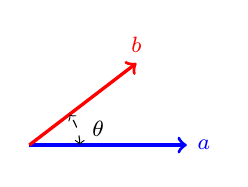
\begin{tikzpicture}[scale=0.8]
    \draw[->,very thick,blue] (0,0) -- (2.5,0) node[right] {\footnotesize $\vect{a}$};
    \draw[->,very thick,red] (0,0) -- (1.7,1.3) node[above] {\footnotesize $\vect{b}$};
    \draw[<->,dashed] (0.8,0) arc (0:37:0.8) node[midway,right,xshift=2pt] {\footnotesize $\theta$};
\end{tikzpicture}
\end{center}
\vspace{0.2cm}

\begin{itemize}
    \item $\theta = 0^\circ$ (same direction): $\cos(0^\circ) = 1$ $\rightarrow$ Dot product is MAX
    \item $\theta = 90^\circ$ (perpendicular): $\cos(90^\circ) = 0$ $\rightarrow$ Dot product is ZERO
    \item $\theta = 180^\circ$ (opposite): $\cos(180^\circ) = -1$ $\rightarrow$ Dot product is NEGATIVE
\end{itemize}

This is why the dot product measures "similarity" or "alignment"!
\end{intuition}

\subsubsection{The Projection Interpretation: Shadows and Flashlights}

Here's another beautiful way to think about the dot product: it measures how much of one vector "falls onto" another.

\begin{intuition}
\textbf{Analogy: The Flashlight and the Wall}

Imagine you're holding a stick (vector $\vect{b}$) and shining a flashlight straight down onto the floor (along vector $\vect{a}$). The shadow of the stick on the floor is the \vocab{projection} of $\vect{b}$ onto $\vect{a}$.

\begin{center}
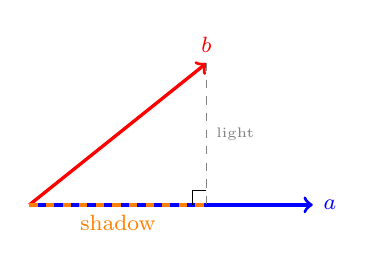
\begin{tikzpicture}[scale=0.9]
    % Floor/a direction
    \draw[->,very thick,blue] (0,0) -- (4,0) node[right] {\footnotesize $\vect{a}$};

    % Vector b
    \draw[->,very thick,red] (0,0) -- (2.5,2) node[above] {\footnotesize $\vect{b}$};

    % Projection (shadow)
    \draw[very thick,orange,dashed] (0,0) -- (2.5,0);
    \node[orange,below] at (1.25,0) {\footnotesize shadow};

    % Vertical dashed line (light rays)
    \draw[dashed,gray] (2.5,2) -- (2.5,0);
    \node[gray,right] at (2.5,1) {\tiny light};

    % Right angle
    \draw (2.5,0.2) -- (2.3,0.2) -- (2.3,0);
\end{tikzpicture}
\end{center}

The dot product $\vect{a} \cdot \vect{b}$ is related to the length of this shadow (scaled by how long $\vect{a}$ is).

\textbf{Why does this matter?}
\begin{itemize}
    \item If $\vect{b}$ points in the same direction as $\vect{a}$: maximum shadow, maximum dot product
    \item If $\vect{b}$ is perpendicular to $\vect{a}$: no shadow at all, dot product is zero!
    \item If $\vect{b}$ points opposite to $\vect{a}$: shadow points backwards, negative dot product
\end{itemize}
\end{intuition}

\subsubsection{Orthogonality: The Magic of Zero}

When the dot product is exactly zero, we say the vectors are \vocab{orthogonal} (fancy word for perpendicular).

\begin{definition}{Orthogonal Vectors}{}
Two vectors $\vect{a}$ and $\vect{b}$ are orthogonal if and only if:
\[
\vect{a} \cdot \vect{b} = 0
\]

They're at right angles to each other---completely unrelated, pointing in independent directions.
\end{definition}

\begin{example}
Check if $[3, 4]$ and $[-4, 3]$ are orthogonal:
\[
[3, 4] \cdot [-4, 3] = (3)(-4) + (4)(3) = -12 + 12 = 0 \quad \checkmark
\]

They're perpendicular! In 2D, you can always make an orthogonal vector by swapping components and negating one: $[a, b] \perp [-b, a]$.
\end{example}

\begin{intuition}
\textbf{Why Orthogonality is Magic}

Orthogonal vectors are completely independent---knowing about one tells you nothing about the other. They're like asking someone their height vs. their favorite color: totally unrelated dimensions of information.

\textbf{Real-world examples of orthogonal concepts:}
\begin{itemize}
    \item North-South vs. East-West (perpendicular directions)
    \item Temperature vs. day of the week (unrelated variables)
    \item In word embeddings: "king" might be orthogonal to "purple" (unrelated concepts)
\end{itemize}

This is why orthogonal bases are so useful---each dimension captures genuinely new information!
\end{intuition}

\begin{connection}
\textbf{This is literally how ChatGPT understands language!}

When you type "The king sat on his throne," the model computes dot products to figure out which words are related:
\begin{itemize}
    \item $\text{``king''} \cdot \text{``throne''}$ → Large! These words appear in similar contexts.
    \item $\text{``king''} \cdot \text{``pizza''}$ → Small. Not really related.
    \item $\text{``king''} \cdot \text{``queen''}$ → Very large! Similar concepts.
\end{itemize}

The entire "attention mechanism" in transformers (the key innovation that makes LLMs work) is built on dot products. Every time ChatGPT decides which words to focus on, it's computing billions of dot products!

\textbf{No joke: The dot product is arguably the most important operation in modern AI.} If you remember one thing from this chapter, remember the dot product. It's everywhere. It's in your phone. It's answering your questions right now.
\end{connection}

\subsubsection{The Famous Word Arithmetic: King - Man + Woman = Queen}

Remember that viral example from 2013 that blew everyone's minds? It actually works because of dot products and the geometry they create!

\begin{example}
\textbf{The Word2Vec Magic Trick}

Researchers discovered that word vectors have this bizarre property:
\[
\text{vector(``king'')} - \text{vector(``man'')} + \text{vector(``woman'')} \approx \text{vector(``queen'')}
\]

How? The vectors encode relationships! Subtracting "man" removes the "male" direction. Adding "woman" adds the "female" direction. What's left? A royal female = queen!

\begin{center}
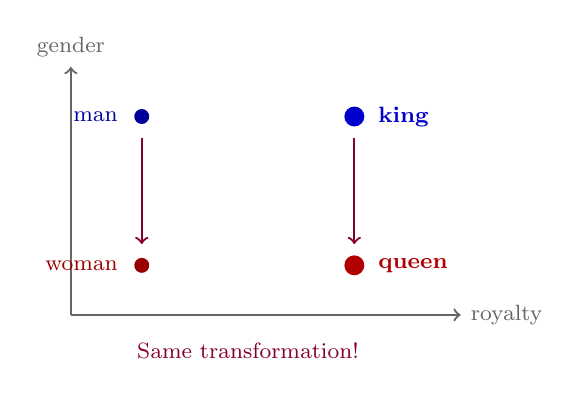
\begin{tikzpicture}[scale=0.9]
    % Axes
    \draw[axis] (0,0) -- (5.5,0) node[right, font=\footnotesize] {royalty};
    \draw[axis] (0,0) -- (0,3.5) node[above, font=\footnotesize] {gender};

    % Words as points with labels
    \fill[blue!80!black] (4,2.8) circle (4pt);
    \node[font=\footnotesize\bfseries, blue!80!black, right] at (4.2,2.8) {king};

    \fill[red!70!black] (4,0.7) circle (4pt);
    \node[font=\footnotesize\bfseries, red!70!black, right] at (4.2,0.7) {queen};

    \fill[blue!60!black] (1,2.8) circle (3pt);
    \node[font=\footnotesize, blue!60!black, left] at (0.8,2.8) {man};

    \fill[red!60!black] (1,0.7) circle (3pt);
    \node[font=\footnotesize, red!60!black, left] at (0.8,0.7) {woman};

    % Transformation arrows
    \draw[->, thick, purple!70!black] (1,2.5) -- (1,1.0);
    \draw[->, thick, purple!70!black] (4,2.5) -- (4,1.0);

    % Annotation
    \node[font=\footnotesize, purple!70!black] at (2.5,-0.5) {Same transformation!};
\end{tikzpicture}
\end{center}

The dot product helps find which word vector is closest to your computed result. It's all vector similarity!
\end{example}

\begin{intuition}
\textbf{Why This Works (The Deep Insight)}

Word embeddings learn to place words so that:
\begin{itemize}
    \item Words with similar meanings have similar vectors (high dot product)
    \item Relationships between words are encoded as consistent directions
    \item "Male to female" is roughly the same direction whether you start at "king," "actor," or "waiter"
\end{itemize}

This emergent structure wasn't programmed---it was learned from reading billions of sentences! The AI discovered that language has this beautiful geometric structure.
\end{intuition}

\subsection{Vector Norms: Measuring How Big Something Is}

Sometimes you need to know: "How big is this vector?" The \vocab{norm} (or \vocab{length}) tells you.

\textbf{Think of it like this:} If a vector is an arrow, the norm is how long the arrow is!

\begin{intuition}
\textbf{Multiple Ways to Measure "Bigness"}

Just like there are different ways to measure distance in real life, there are different norms:

\begin{itemize}
    \item \textbf{$L^2$ norm (Euclidean):} "As the crow flies" distance. The straight-line path.
    \item \textbf{$L^1$ norm (Manhattan):} "City block" distance. How far you'd walk if you could only go along streets (no cutting through buildings).
    \item \textbf{$L^\infty$ norm (Max):} "What's the biggest single step?" Only looks at the largest component.
\end{itemize}

\begin{center}
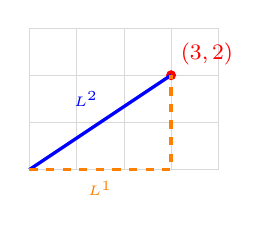
\begin{tikzpicture}[scale=0.6]
    % Grid
    \draw[very thin,gray!30] (0,0) grid (4,3);

    % Point
    \fill[red] (3,2) circle (3pt);
    \node[red,above right] at (3,2) {\footnotesize $(3,2)$};

    % L2 (straight line)
    \draw[very thick,blue] (0,0) -- (3,2);
    \node[blue] at (1.2,1.5) {\tiny $L^2$};

    % L1 (city blocks)
    \draw[very thick,orange,dashed] (0,0) -- (3,0) -- (3,2);
    \node[orange] at (1.5,-0.4) {\tiny $L^1$};
\end{tikzpicture}
\end{center}

For the point $(3, 2)$:
\begin{itemize}
    \item $L^2$ distance: $\sqrt{3^2 + 2^2} = \sqrt{13} \approx 3.6$ (diagonal)
    \item $L^1$ distance: $|3| + |2| = 5$ (walking the streets)
    \item $L^\infty$ distance: $\max(|3|, |2|) = 3$ (biggest coordinate)
\end{itemize}
\end{intuition}

\vspace{0.3cm}
\begin{center}
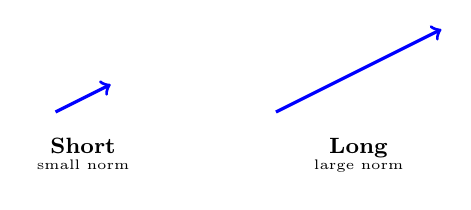
\begin{tikzpicture}[scale=0.7]
    % Short vector (left)
    \begin{scope}
    \draw[->,very thick,blue] (0,0) -- (1,0.5);
    \node[below] at (0.5,-0.3) {\footnotesize \textbf{Short}};
    \node[below] at (0.5,-0.7) {\tiny small norm};
    \end{scope}

    % Long vector (right)
    \begin{scope}[xshift=4cm]
    \draw[->,very thick,blue] (0,0) -- (3,1.5);
    \node[below] at (1.5,-0.3) {\footnotesize \textbf{Long}};
    \node[below] at (1.5,-0.7) {\tiny large norm};
    \end{scope}
\end{tikzpicture}
\end{center}
\vspace{0.3cm}

\begin{definition}{Vector Norm (Length)}{}
The \vocab{$L^2$ norm} (also called Euclidean norm) is:
\[
\norm{\vect{v}} = \sqrt{v_1^2 + v_2^2 + \cdots + v_n^2} = \sqrt{\sum_{i=1}^{n} v_i^2}
\]

It's basically the Pythagorean theorem extended to any number of dimensions!
\end{definition}

\begin{example}
For $\vect{v} = [3, 4]$:
\[
\norm{\vect{v}} = \sqrt{3^2 + 4^2} = \sqrt{9 + 16} = \sqrt{25} = 5
\]

For $\vect{w} = [1, 2, 2]$:
\[
\norm{\vect{w}} = \sqrt{1^2 + 2^2 + 2^2} = \sqrt{1 + 4 + 4} = \sqrt{9} = 3
\]
\end{example}

\begin{intuition}
\textbf{For 2D vectors, it's just the Pythagorean theorem!}

For $\vect{v} = [3, 4]$:

\vspace{0.3cm}
\begin{center}
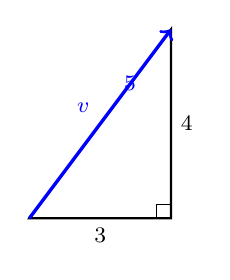
\begin{tikzpicture}[scale=0.6]
    % Right triangle
    \draw[thick] (0,0) -- (3,0) -- (3,4) -- cycle;
    \draw[->,very thick,blue] (0,0) -- (3,4) node[midway,above left] {\footnotesize $\vect{v}$};

    % Labels
    \node[below] at (1.5,0) {\footnotesize 3};
    \node[right] at (3,2) {\footnotesize 4};
    \node[above right,blue] at (1.8,2.5) {\footnotesize 5};

    % Right angle marker
    \draw (3,0.3) -- (2.7,0.3) -- (2.7,0);
\end{tikzpicture}
\end{center}
\textit{Good old Pythagoras! $\sqrt{3^2 + 4^2} = \sqrt{25} = 5$}
\vspace{0.3cm}

You go 3 steps right and 4 steps up. The straight-line distance is 5!

\textbf{In 3D:} $\text{length} = \sqrt{x^2 + y^2 + z^2}$

\textbf{In any dimension:} Square each component, add them up, take the square root!

\textbf{Physical meaning:} How far are you from where you started (the origin)?
\end{intuition}

\begin{connection}
\textbf{Why LLMs care about length:}

When comparing word vectors, we often don't want the comparison to depend on how "loud" the vector is. A whisper of "king" and a shout of "king" should mean the same thing.

So we often normalize vectors (make them length 1) before comparing them. This way, we only care about the \textit{direction} of the vector, not its magnitude.
\end{connection}

\subsection{Unit Vectors: Keeping Only Direction}

A \vocab{unit vector} is a vector with length exactly 1. It only encodes direction, not magnitude.

\begin{definition}{Normalization}{}
To convert any vector into a unit vector pointing in the same direction, divide by its norm:
\[
\hat{\vect{v}} = \frac{\vect{v}}{\norm{\vect{v}}}
\]

The hat symbol ($\hat{\phantom{v}}$) means "unit vector version of."
\end{definition}

\begin{example}
Let's normalize $\vect{v} = [3, 4]$:

First, find its length: $\norm{\vect{v}} = 5$ (we calculated this earlier)

Then divide:
\[
\hat{\vect{v}} = \frac{1}{5} \begin{bmatrix} 3 \\ 4 \end{bmatrix} = \begin{bmatrix} 0.6 \\ 0.8 \end{bmatrix}
\]

Check: $\norm{\hat{\vect{v}}} = \sqrt{0.6^2 + 0.8^2} = \sqrt{0.36 + 0.64} = \sqrt{1} = 1$ \checkmark
\end{example}

\begin{connection}
\textbf{In transformers:}

Before computing attention scores (those dot products we talked about), the model often normalizes the vectors. This makes the attention mechanism more stable and prevents numbers from getting too large or too small.

It's like adjusting everyone to speak at the same volume before having a conversation—you can focus on \textit{what} they're saying, not \textit{how loud} they are.
\end{connection}

\section{Matrices: Tables of Numbers That Transform Reality}

Vectors are lists. Matrices are \textit{tables}. That's the only difference.

But here's where it gets exciting: while vectors \textit{are} data, matrices \textit{do things} to data. A matrix is an action, a transformation, a function waiting to happen. When you multiply a matrix by a vector, you're not just doing arithmetic---you're transforming reality itself (mathematically speaking).

\subsection{What IS a Matrix?}

A \vocab{matrix} is a rectangular grid of numbers. It has rows (horizontal) and columns (vertical). Think of it as a spreadsheet, or a table, or a grid of values.

\begin{intuition}
\textbf{Two Ways to Think About Matrices}

\textbf{1. As a table of data:}
A matrix can just store information. Student grades, pixel values in an image, connection strengths between neurons.

\textbf{2. As a transformation machine:}
A matrix can \textit{do something} to vectors. Rotate them, stretch them, project them, mix their components around.

Both views are valid! Sometimes a matrix is just data. Sometimes it's an operation. The math doesn't care which interpretation you use---it works the same either way. This dual nature is part of what makes matrices so powerful.
\end{intuition}

\begin{definition}{Matrix}{}
An $m \times n$ matrix has $m$ rows and $n$ columns:
\[
\mat{A} = \begin{bmatrix}
a_{11} & a_{12} & \cdots & a_{1n} \\
a_{21} & a_{22} & \cdots & a_{2n} \\
\vdots & \vdots & \ddots & \vdots \\
a_{m1} & a_{m2} & \cdots & a_{mn}
\end{bmatrix}
\]

We say $\mat{A} \in \R^{m \times n}$ (a table with $m$ rows and $n$ columns of real numbers).
\end{definition}

\begin{example}
Here's a $2 \times 3$ matrix (2 rows, 3 columns):
\[
\mat{A} = \begin{bmatrix}
1 & 2 & 3 \\
4 & 5 & 6
\end{bmatrix}
\]

Here's a $3 \times 2$ matrix (3 rows, 2 columns):
\[
\mat{B} = \begin{bmatrix}
7 & 8 \\
9 & 10 \\
11 & 12
\end{bmatrix}
\]

Here's a $4 \times 4$ matrix (a square matrix):
\[
\mat{C} = \begin{bmatrix}
1 & 0 & 0 & 0 \\
0 & 2 & 0 & 0 \\
0 & 0 & 3 & 0 \\
0 & 0 & 0 & 4
\end{bmatrix}
\]
\end{example}

\textbf{Real-world matrices are EVERYWHERE:}
\begin{itemize}
    \item \textbf{Spreadsheet:} Each cell has a number. That's a matrix!
    \item \textbf{Image:} A 1920×1080 image is a matrix with 1080 rows and 1920 columns of pixel brightness values. Color images are three matrices stacked (one each for red, green, blue)!
    \item \textbf{Social network:} A matrix where row $i$, column $j$ = 1 if person $i$ follows person $j$. Twitter's "who follows whom" is a giant matrix with billions of entries!
    \item \textbf{Student grades:} Rows = students, columns = assignments, values = grades
    \item \textbf{Game state:} A chess board is an 8×8 matrix. Sudoku is a 9×9 matrix. Minecraft chunks are 3D matrices (tensors)!
    \item \textbf{Word co-occurrence:} A matrix where entry $(i,j)$ counts how often word $i$ appears near word $j$. This was how early word embeddings were created!
\end{itemize}

\begin{connection}
\textbf{Neural Networks Are Stacks of Matrices}

Here's the mind-blowing truth: a neural network is basically a sequence of matrices. Each layer has a weight matrix. Training the network means adjusting the numbers in these matrices.

GPT-4 has about 1.8 trillion parameters---numbers stored in matrices. When you chat with an AI, you're watching these matrices transform your input, layer by layer, until language emerges.

Every clever thing AI does? Matrix multiplication. Every "emergent ability"? Matrix multiplication (plus some nonlinear functions). It's matrices all the way down.
\end{connection}

\subsection{Matrix-Vector Multiplication: Transforming Space Itself}

Here's where things get REALLY wild. When you multiply a matrix by a vector, you're \textit{transforming} that vector. You're pushing it around, rotating it, stretching it, squishing it.

\textbf{Think of matrices as TRANSFORMATION MACHINES:}

\vspace{0.3cm}
\begin{center}
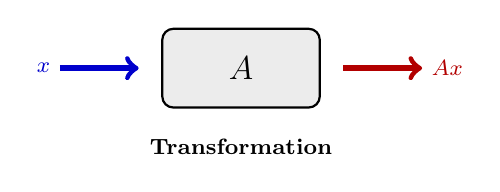
\begin{tikzpicture}[scale=1.0]
    % Input vector
    \draw[vec blue, line width=2pt] (-0.3,0.5) -- (0.7,0.5);
    \node[left, blue!80!black, font=\footnotesize] at (-0.3,0.5) {$\vect{x}$};

    % Transformation box
    \draw[thick, rounded corners=4pt, fill=gray!15] (1,0) rectangle (3,1);
    \node[font=\large] at (2,0.5) {$\mat{A}$};

    % Output vector
    \draw[vec red, line width=2pt] (3.3,0.5) -- (4.3,0.5);
    \node[right, red!70!black, font=\footnotesize] at (4.3,0.5) {$\mat{A}\vect{x}$};

    % Title
    \node[font=\footnotesize\bfseries] at (2,-0.5) {Transformation};
\end{tikzpicture}
\end{center}
\vspace{0.2cm}
\textit{Put a vector in, get a (possibly different) vector out. That's matrix multiplication!}
\vspace{0.3cm}

\textbf{The Big Idea:} A matrix is like a function. Input goes in, output comes out. But unlike arbitrary functions, matrices are "linear"---they can only do certain types of transformations (stretching, rotating, shearing, projecting). They can't do "curvy" things. This limitation is actually a superpower: it makes them predictable, analyzable, and efficient to compute.

\textbf{Let's see it in action with a simple example:}

\begin{definition}{Matrix-Vector Multiplication}{}
If $\mat{A}$ is $m \times n$ and $\vect{x}$ is $n \times 1$, then $\mat{A}\vect{x}$ is an $m \times 1$ vector:
\[
\mat{A}\vect{x} = \begin{bmatrix}
\text{(row 1 of } \mat{A}) \cdot \vect{x} \\
\text{(row 2 of } \mat{A}) \cdot \vect{x} \\
\vdots \\
\text{(row } m \text{ of } \mat{A}) \cdot \vect{x}
\end{bmatrix}
\]

Each component of the result is the dot product of a row of $\mat{A}$ with $\vect{x}$.
\end{definition}

\begin{example}
Let's compute:
\begin{align*}
\begin{bmatrix}
1 & 2 \\
3 & 4 \\
5 & 6
\end{bmatrix}
\begin{bmatrix}
7 \\
8
\end{bmatrix}
&= \begin{bmatrix}
(1)(7) + (2)(8) \\
(3)(7) + (4)(8) \\
(5)(7) + (6)(8)
\end{bmatrix} \\[0.5em]
&= \begin{bmatrix}
7 + 16 \\
21 + 32 \\
35 + 48
\end{bmatrix}
= \begin{bmatrix}
23 \\
53 \\
83
\end{bmatrix}
\end{align*}

We started with a 2D vector $[7, 8]$ and got a 3D vector $[23, 53, 83]$! The matrix transformed it from 2D to 3D!
\end{example}

\textbf{THE GEOMETRIC VIEW (This is Beautiful!):}

Matrices don't just change individual vectors—they transform ENTIRE SPACE! Let's see what different matrices actually DO:

\textbf{1. Scaling Matrix (Stretch/Shrink):}

\vspace{0.3cm}
\begin{center}
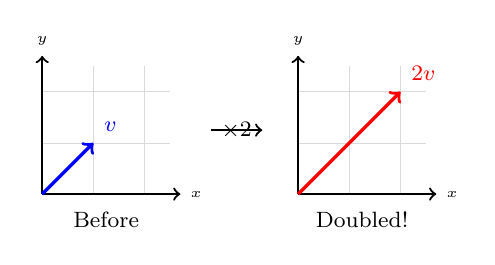
\begin{tikzpicture}[scale=0.65]
    % Before
    \begin{scope}
        \draw[very thin,gray!30] (0,0) grid (2.5,2.5);
        \draw[->,thick] (0,0) -- (2.7,0) node[right] {\tiny $x$};
        \draw[->,thick] (0,0) -- (0,2.7) node[above] {\tiny $y$};
        \draw[->,very thick,blue] (0,0) -- (1,1) node[above right] {\footnotesize $\vect{v}$};
        \node at (1.25,-0.5) {\footnotesize Before};
    \end{scope}

    % Arrow
    \node at (3.8,1.25) {\footnotesize $\times 2$};
    \draw[->,thick] (3.3,1.25) -- (4.3,1.25);

    % After
    \begin{scope}[xshift=5cm]
        \draw[very thin,gray!30] (0,0) grid (2.5,2.5);
        \draw[->,thick] (0,0) -- (2.7,0) node[right] {\tiny $x$};
        \draw[->,thick] (0,0) -- (0,2.7) node[above] {\tiny $y$};
        \draw[->,very thick,red] (0,0) -- (2,2) node[above right] {\footnotesize $2\vect{v}$};
        \node at (1.25,-0.5) {\footnotesize Doubled!};
    \end{scope}
\end{tikzpicture}
\end{center}
\vspace{0.3cm}

\textbf{2. Rotation Matrix (Spin Around):}

\vspace{0.3cm}
\begin{center}
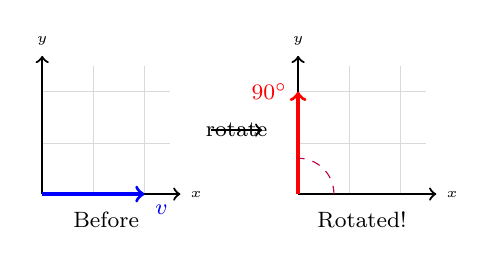
\begin{tikzpicture}[scale=0.65]
    % Before
    \begin{scope}
        \draw[very thin,gray!30] (0,0) grid (2.5,2.5);
        \draw[->,thick] (0,0) -- (2.7,0) node[right] {\tiny $x$};
        \draw[->,thick] (0,0) -- (0,2.7) node[above] {\tiny $y$};
        \draw[->,very thick,blue] (0,0) -- (2,0) node[below right] {\footnotesize $\vect{v}$};
        \node at (1.25,-0.5) {\footnotesize Before};
    \end{scope}

    % Arrow
    \node at (3.8,1.25) {\footnotesize rotate};
    \draw[->,thick] (3.3,1.25) -- (4.3,1.25);

    % After
    \begin{scope}[xshift=5cm]
        \draw[very thin,gray!30] (0,0) grid (2.5,2.5);
        \draw[->,thick] (0,0) -- (2.7,0) node[right] {\tiny $x$};
        \draw[->,thick] (0,0) -- (0,2.7) node[above] {\tiny $y$};
        \draw[->,very thick,red] (0,0) -- (0,2) node[left] {\footnotesize $90^\circ$};
        \draw[dashed,purple] (0.7,0) arc (0:90:0.7);
        \node at (1.25,-0.5) {\footnotesize Rotated!};
    \end{scope}
\end{tikzpicture}
\end{center}
\vspace{0.3cm}

\textbf{3. Shear Matrix (Slant/Skew):}

\vspace{0.3cm}
\begin{center}
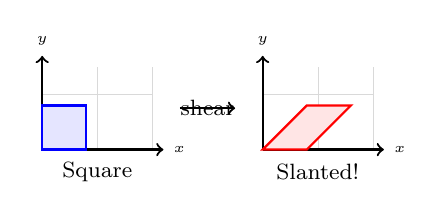
\begin{tikzpicture}[scale=0.7]
    % Before
    \begin{scope}
        \draw[very thin,gray!30] (0,0) grid (2,1.5);
        \draw[->,thick] (0,0) -- (2.2,0) node[right] {\tiny $x$};
        \draw[->,thick] (0,0) -- (0,1.7) node[above] {\tiny $y$};
        \draw[thick,blue,fill=blue!10] (0,0) rectangle (0.8,0.8);
        \node at (1,-0.4) {\footnotesize Square};
    \end{scope}

    % Arrow
    \node at (3,0.75) {\footnotesize shear};
    \draw[->,thick] (2.5,0.75) -- (3.5,0.75);

    % After
    \begin{scope}[xshift=4cm]
        \draw[very thin,gray!30] (0,0) grid (2,1.5);
        \draw[->,thick] (0,0) -- (2.2,0) node[right] {\tiny $x$};
        \draw[->,thick] (0,0) -- (0,1.7) node[above] {\tiny $y$};
        \draw[thick,red,fill=red!10] (0,0) -- (0.8,0) -- (1.6,0.8) -- (0.8,0.8) -- cycle;
        \node at (1,-0.4) {\footnotesize Slanted!};
    \end{scope}
\end{tikzpicture}
\end{center}
\vspace{0.2cm}
\textit{Like pushing a deck of cards sideways!}
\vspace{0.3cm}

\begin{intuition}
\textbf{The Key Insight:} A matrix doesn't just move one vector—it transforms the ENTIRE COORDINATE SYSTEM!

Think of it like Instagram filters:
\begin{itemize}
    \item Input: Your photo (represented as vectors of pixels)
    \item Matrix: The filter transformation
    \item Output: Filtered photo (transformed vectors)
\end{itemize}

\textbf{What matrices can do:}
\begin{itemize}
    \item \textbf{Rotate:} Spin things around
    \item \textbf{Scale:} Make things bigger or smaller
    \item \textbf{Shear:} Slant things (like pushing a deck of cards)
    \item \textbf{Reflect:} Flip things (mirror image)
    \item \textbf{Project:} Flatten 3D onto 2D (like a shadow)
    \item \textbf{Combinations:} Mix any of the above!
\end{itemize}

\textbf{Mind-blowing fact:} Every linear transformation (rotation, scaling, shearing, etc.) can be represented as a matrix! That's why matrices are so powerful! And every matrix \textit{is} a transformation. They're two sides of the same coin.

\textbf{The Secret Decoder Ring:} Want to know what a $2 \times 2$ matrix does? Just look at where it sends the standard basis vectors $[1, 0]$ and $[0, 1]$:
\begin{itemize}
    \item Column 1 of the matrix = where $[1, 0]$ goes
    \item Column 2 of the matrix = where $[0, 1]$ goes
\end{itemize}

This tells you everything! If $[1, 0]$ maps to $[2, 0]$ (doubled) and $[0, 1]$ maps to $[0, 3]$ (tripled), the matrix stretches x by 2 and y by 3.
\end{intuition}

\begin{example}
\textbf{Decoding Common Transformation Matrices}

\textbf{Rotation by 90 degrees counterclockwise:}
\[
\mat{R}_{90} = \begin{bmatrix}
0 & -1 \\
1 & 0
\end{bmatrix}
\]
Check: $[1, 0] \rightarrow [0, 1]$ (right arrow points up now) and $[0, 1] \rightarrow [-1, 0]$ (up arrow points left now). That's a 90-degree rotation!

\textbf{Horizontal flip (mirror):}
\[
\mat{F} = \begin{bmatrix}
-1 & 0 \\
0 & 1
\end{bmatrix}
\]
Check: $[1, 0] \rightarrow [-1, 0]$ (right becomes left) and $[0, 1] \rightarrow [0, 1]$ (up stays up). Mirror across the y-axis!

\textbf{Projection onto the x-axis:}
\[
\mat{P} = \begin{bmatrix}
1 & 0 \\
0 & 0
\end{bmatrix}
\]
Check: $[1, 0] \rightarrow [1, 0]$ and $[0, 1] \rightarrow [0, 0]$. Everything gets squashed onto the x-axis! (This is a rank-1 matrix---notice how it destroys the y-dimension.)
\end{example}

\begin{connection}
\textbf{Neural networks are just matrix multiplications!}

When you hear "neural network," think: a series of matrix-vector multiplications, with some nonlinear functions sprinkled in between.

A simple neural network layer looks like:
\[
\text{output} = \text{activation}(\mat{W} \times \text{input} + \vect{b})
\]

Where:
\begin{itemize}
    \item $\mat{W}$ is a matrix of "weights" (the learned parameters)
    \item $\text{input}$ is your input vector (maybe word embeddings)
    \item $\vect{b}$ is a "bias" vector (more learned parameters)
    \item $\text{activation}$ is a nonlinear function (like ReLU or sigmoid)
\end{itemize}

That's it! Stack a dozen of these together, and you have GPT.
\end{connection}

\subsection{Matrix-Matrix Multiplication: Composing Transformations}

What if you want to apply two transformations in sequence? First rotate, then scale? First shear, then reflect?

Here's the magical answer: \textbf{multiply the matrices together!} The result is a single matrix that does both transformations at once.

\begin{intuition}
\textbf{Analogy: Instagram Filters}

Imagine you apply the "Vintage" filter to a photo, then apply "Brighten." Instead of applying two separate operations, Instagram could mathematically combine them into a single "Vintage+Brighten" filter that does both at once.

That's exactly what matrix multiplication does! If $\mat{A}$ is "Vintage" and $\mat{B}$ is "Brighten," then $\mat{B}\mat{A}$ is "Apply Vintage, then Brighten" as a single operation.

\textbf{Why this matters for AI:} Neural networks do this all the time. Instead of applying 100 layers separately, you could (in theory) multiply all the weight matrices together into one giant matrix. (In practice, we don't do this because the nonlinear activation functions between layers prevent it---but mathematically, the linear parts compose beautifully.)
\end{intuition}

\begin{definition}{Matrix-Matrix Multiplication}{}
If $\mat{A}$ is $m \times n$ and $\mat{B}$ is $n \times p$, then $\mat{A}\mat{B}$ is $m \times p$:
\[
(\mat{A}\mat{B})_{ij} = \text{(row } i \text{ of } \mat{A}) \cdot \text{(column } j \text{ of } \mat{B})
\]

Entry $(i,j)$ of the result is the dot product of row $i$ from $\mat{A}$ and column $j$ from $\mat{B}$.
\end{definition}

\begin{example}
Multiply a $2 \times 3$ matrix by a $3 \times 2$ matrix:
\[
\begin{bmatrix}
1 & 2 & 3 \\
4 & 5 & 6
\end{bmatrix}
\begin{bmatrix}
7 & 8 \\
9 & 10 \\
11 & 12
\end{bmatrix}
\]

Result will be $2 \times 2$. Let's compute:
\begin{itemize}
    \item Top-left: $(1, 2, 3) \cdot (7, 9, 11) = 7 + 18 + 33 = 58$
    \item Top-right: $(1, 2, 3) \cdot (8, 10, 12) = 8 + 20 + 36 = 64$
    \item Bottom-left: $(4, 5, 6) \cdot (7, 9, 11) = 28 + 45 + 66 = 139$
    \item Bottom-right: $(4, 5, 6) \cdot (8, 10, 12) = 32 + 50 + 72 = 154$
\end{itemize}

So:
\[
\begin{bmatrix}
1 & 2 & 3 \\
4 & 5 & 6
\end{bmatrix}
\begin{bmatrix}
7 & 8 \\
9 & 10 \\
11 & 12
\end{bmatrix}
= \begin{bmatrix}
58 & 64 \\
139 & 154
\end{bmatrix}
\]
\end{example}

\textbf{Important facts about matrix multiplication:}
\begin{itemize}
    \item \textbf{Not commutative:} $\mat{A}\mat{B} \neq \mat{B}\mat{A}$ (order matters!)
    \item \textbf{Associative:} $(\mat{A}\mat{B})\mat{C} = \mat{A}(\mat{B}\mat{C})$
    \item \textbf{Size rule:} $(m \times n) \times (n \times p) = (m \times p)$. The inner dimensions must match!
\end{itemize}

\begin{intuition}
\textbf{Why Isn't Matrix Multiplication Commutative?}

This trips people up, so let's really understand it. Think about getting dressed:
\begin{itemize}
    \item Put on socks, then put on shoes = Normal day
    \item Put on shoes, then put on socks = You look ridiculous
\end{itemize}

Order matters for getting dressed. Order matters for matrices.

Geometrically: ``Rotate $90^\circ$, then scale by 2'' gives a different result than ``Scale by 2, then rotate $90^\circ$''. Well, actually for these specific transforms it's the same---but try ``shear, then rotate'' vs ``rotate, then shear'' and you'll get totally different results!

\textbf{Real example:}
\[
\begin{bmatrix} 1 & 2 \\ 0 & 1 \end{bmatrix}
\begin{bmatrix} 0 & 1 \\ 1 & 0 \end{bmatrix}
= \begin{bmatrix} 2 & 1 \\ 1 & 0 \end{bmatrix}
\quad \text{but} \quad
\begin{bmatrix} 0 & 1 \\ 1 & 0 \end{bmatrix}
\begin{bmatrix} 1 & 2 \\ 0 & 1 \end{bmatrix}
= \begin{bmatrix} 0 & 1 \\ 1 & 2 \end{bmatrix}
\]

Different results! The first does "flip axes, then shear." The second does "shear, then flip axes."
\end{intuition}

\begin{connection}
\textbf{Deep learning is deep matrix multiplication:}

A neural network with 10 layers applies 10 matrix transformations in sequence. If each layer has weight matrix $\mat{W}_i$, the full network computes:
\[
\mat{W}_{10} \times \mat{W}_9 \times \cdots \times \mat{W}_2 \times \mat{W}_1 \times \text{input}
\]

Each matrix transforms the data a little, and together they transform raw pixels into "this is a cat" or random text into "this is a coherent sentence."
\end{connection}

\subsection{The Transpose: Flipping Rows and Columns}

The \vocab{transpose} of a matrix swaps its rows and columns. It's like rotating a spreadsheet 90 degrees and then flipping it!

\begin{intuition}
\textbf{Why Does the Transpose Exist?}

At first, swapping rows and columns seems like a random operation. Why would anyone want to do this?

Here are some reasons the transpose is secretly everywhere:

\textbf{1. Dot products as matrix multiplication:} Remember the dot product? $\vect{a} \cdot \vect{b}$? It can be written as $\vect{a}^\top \vect{b}$ (row vector times column vector). This unifies dot products with matrix multiplication!

\textbf{2. "From" vs "To":} If matrix $\mat{A}$ transforms from space X to space Y, then $\mat{A}^\top$ often relates Y back to X. It's like having a map and its reverse.

\textbf{3. Gradients in neural networks:} During backpropagation, you constantly use transposes. If the forward pass multiplies by $\mat{W}$, the backward pass multiplies by $\mat{W}^\top$. This isn't a coincidence---it's deep math!

\textbf{4. Symmetry detection:} A matrix equals its transpose ($\mat{A} = \mat{A}^\top$) if and only if it's symmetric. The transpose is how we check for this important property.
\end{intuition}

\textbf{Visual representation:}

\vspace{0.3cm}
\begin{center}
\begin{tikzpicture}[scale=0.7]
    % Original matrix
    \node at (0,1.5) {\footnotesize $\mat{A} = \begin{bmatrix} 1 & 2 & 3 \\ 4 & 5 & 6 \end{bmatrix}$};

    % Arrow showing flip
    \draw[->,thick,blue] (1.8,0.8) -- (2.8,0.8);
    \node[blue,above] at (2.3,0.8) {\tiny flip};

    % Transposed
    \node at (4.5,1.5) {\footnotesize $\mat{A}^\top = \begin{bmatrix} 1 & 4 \\ 2 & 5 \\ 3 & 6 \end{bmatrix}$};

    \begin{scope}[xshift=4cm]
        \draw[thick] (0,0) grid[step=0.5] (1,1.5);
        \node at (0.25,1.25) {\tiny 1};
        \node at (0.75,1.25) {\tiny 4};
        \node at (0.25,0.75) {\tiny 2};
        \node at (0.75,0.75) {\tiny 5};
        \node at (0.25,0.25) {\tiny 3};
        \node at (0.75,0.25) {\tiny 6};
    \end{scope}

    \node at (2.5,-0.8) {\small \textbf{Rows $\leftrightarrow$ columns}};
\end{tikzpicture}
\end{center}
\vspace{0.3cm}

\begin{definition}{Matrix Transpose}{}
If $\mat{A}$ is $m \times n$, then $\mat{A}^\top$ (read: "A transpose") is $n \times m$ where:
\[
(\mat{A}^\top)_{ij} = \mat{A}_{ji}
\]

The rows of $\mat{A}$ become the columns of $\mat{A}^\top$.
\end{definition}

\begin{example}
\[
\mat{A} = \begin{bmatrix}
1 & 2 & 3 \\
4 & 5 & 6
\end{bmatrix}_{2 \times 3}
\quad \Rightarrow \quad
\mat{A}^\top = \begin{bmatrix}
1 & 4 \\
2 & 5 \\
3 & 6
\end{bmatrix}_{3 \times 2}
\]

For a vector:
\[
\vect{v} = \begin{bmatrix} 1 \\ 2 \\ 3 \end{bmatrix}
\quad \Rightarrow \quad
\vect{v}^\top = \begin{bmatrix} 1 & 2 & 3 \end{bmatrix}
\]

(Column vector becomes row vector)
\end{example}

\textbf{Cool properties:}
\begin{itemize}
    \item $(\mat{A}^\top)^\top = \mat{A}$ (transpose twice, back to original)
    \item $(\mat{A} + \mat{B})^\top = \mat{A}^\top + \mat{B}^\top$
    \item $(\mat{A}\mat{B})^\top = \mat{B}^\top \mat{A}^\top$ (order reverses!)
    \item $\vect{a} \cdot \vect{b} = \vect{a}^\top \vect{b}$ (dot product as matrix multiplication)
\end{itemize}

\begin{connection}
\textbf{In neural networks:}

The transpose shows up \textit{everywhere}. When computing gradients (how to update weights during learning), you often need to transpose matrices. The backpropagation algorithm (which we'll cover later) is full of transposes.

Also, the dot product $\vect{a} \cdot \vect{b}$ is often written as $\vect{a}^\top \vect{b}$ because it's technically matrix multiplication of a $1 \times n$ matrix with an $n \times 1$ matrix.
\end{connection}

\section{Special Matrices: The VIPs of Linear Algebra}

Some matrices are special and show up everywhere. Let's meet them!

\subsection{The Identity Matrix: The "Do Nothing" Matrix}

The \vocab{identity matrix} $\mat{I}$ is like multiplying by 1—it doesn't change anything. It's the laziest matrix ever!

\textbf{Geometric View: The Identity Matrix Does NOTHING}

\vspace{0.3cm}
\begin{center}
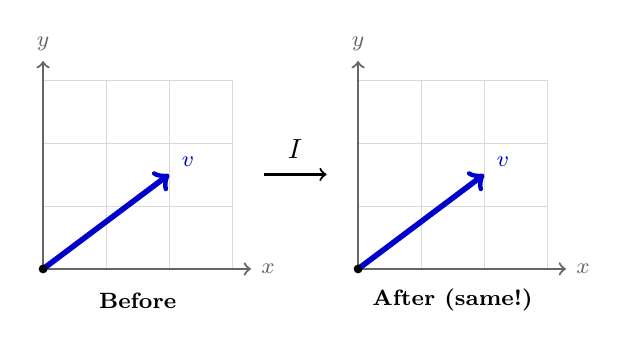
\begin{tikzpicture}[scale=0.8]
    % Before
    \begin{scope}
        \draw[grid] (0,0) grid (3,3);
        \draw[axis] (0,0) -- (3.3,0) node[right, font=\footnotesize] {$x$};
        \draw[axis] (0,0) -- (0,3.3) node[above, font=\footnotesize] {$y$};
        \draw[vec blue, line width=2pt] (0,0) -- (2,1.5);
        \node[blue!80!black, font=\footnotesize] at (2.3,1.7) {$\vect{v}$};
        \fill[black] (0,0) circle (2pt);
        \node[font=\footnotesize\bfseries] at (1.5,-0.5) {Before};
    \end{scope}

    % Arrow
    \draw[->, thick] (3.5,1.5) -- (4.5,1.5);
    \node[font=\normalsize] at (4,1.9) {$\mat{I}$};

    % After
    \begin{scope}[xshift=5cm]
        \draw[grid] (0,0) grid (3,3);
        \draw[axis] (0,0) -- (3.3,0) node[right, font=\footnotesize] {$x$};
        \draw[axis] (0,0) -- (0,3.3) node[above, font=\footnotesize] {$y$};
        \draw[vec blue, line width=2pt] (0,0) -- (2,1.5);
        \node[blue!80!black, font=\footnotesize] at (2.3,1.7) {$\vect{v}$};
        \fill[black] (0,0) circle (2pt);
        \node[font=\footnotesize\bfseries] at (1.5,-0.5) {After (same!)};
    \end{scope}
\end{tikzpicture}
\end{center}
\vspace{0.3cm}

\begin{definition}{Identity Matrix}{}
The $n \times n$ identity matrix has 1s on the diagonal and 0s everywhere else:
\[
\mat{I}_n = \begin{bmatrix}
1 & 0 & \cdots & 0 \\
0 & 1 & \cdots & 0 \\
\vdots & \vdots & \ddots & \vdots \\
0 & 0 & \cdots & 1
\end{bmatrix}
\]

For any matrix $\mat{A}$: $\mat{I}\mat{A} = \mat{A}\mat{I} = \mat{A}$

For any vector $\vect{v}$: $\mat{I}\vect{v} = \vect{v}$
\end{definition}

\begin{example}
\[
\mat{I}_3 = \begin{bmatrix}
1 & 0 & 0 \\
0 & 1 & 0 \\
0 & 0 & 1
\end{bmatrix}
\]

Multiply it by anything:
\[
\begin{bmatrix}
1 & 0 & 0 \\
0 & 1 & 0 \\
0 & 0 & 1
\end{bmatrix}
\begin{bmatrix}
5 \\
7 \\
9
\end{bmatrix}
= \begin{bmatrix}
5 \\
7 \\
9
\end{bmatrix}
\]

Nothing changed! It's the "do nothing" matrix.
\end{example}

\subsection{Diagonal Matrices: The Independent Scalers}

A \vocab{diagonal matrix} has numbers on the main diagonal and zeros everywhere else. They're beautifully simple---and secretly, they're the goal of most matrix decompositions!

\textbf{Why diagonal matrices are amazing:}
\begin{itemize}
    \item \textbf{Easy to understand:} Each dimension is scaled independently
    \item \textbf{Easy to compute:} Multiplication is just component-wise scaling
    \item \textbf{Easy to invert:} Just flip each diagonal element (if non-zero)
    \item \textbf{Easy to raise to powers:} $\mat{D}^n$ = raise each diagonal element to $n$th power
\end{itemize}

Much of advanced linear algebra (eigendecomposition, SVD) is about finding ways to "secretly" turn complicated matrices into diagonal ones!

\textbf{Geometric View: Diagonal Matrices Stretch Each Axis Independently}

\vspace{0.3cm}
\begin{center}
\begin{tikzpicture}[scale=0.85]
    % Before
    \begin{scope}
        \draw[grid] (0,0) grid (3,2);
        \draw[axis] (0,0) -- (3.4,0) node[right, font=\footnotesize] {$x$};
        \draw[axis] (0,0) -- (0,2.4) node[above, font=\footnotesize] {$y$};

        % Unit square
        \fill[blue!20] (0,0) rectangle (1,1);
        \draw[blue!70!black, thick] (0,0) rectangle (1,1);

        \fill[black] (0,0) circle (2pt);
        \node[font=\footnotesize\bfseries] at (1.5,-0.5) {Unit square};
    \end{scope}

    % Arrow with matrix
    \draw[->, thick] (3.6,1) -- (4.8,1);
    \node[font=\small] at (4.2,1.6) {$\begin{bmatrix} 3 & 0 \\ 0 & 2 \end{bmatrix}$};

    % After
    \begin{scope}[xshift=5.2cm]
        \draw[grid] (0,0) grid (3,2);
        \draw[axis] (0,0) -- (3.4,0) node[right, font=\footnotesize] {$x$};
        \draw[axis] (0,0) -- (0,2.4) node[above, font=\footnotesize] {$y$};

        % Stretched rectangle
        \fill[red!20] (0,0) rectangle (3,2);
        \draw[red!70!black, thick] (0,0) rectangle (3,2);

        \fill[black] (0,0) circle (2pt);
        \node[font=\footnotesize\bfseries] at (1.5,-0.5) {3x wide, 2x tall};
    \end{scope}
\end{tikzpicture}
\end{center}
\vspace{0.3cm}

\textbf{Key insight:} Diagonal matrices scale each dimension independently! No rotation, no shearing—just pure stretching or shrinking along axes.

\begin{definition}{Diagonal Matrix}{}
\[
\mat{D} = \begin{bmatrix}
d_1 & 0 & \cdots & 0 \\
0 & d_2 & \cdots & 0 \\
\vdots & \vdots & \ddots & \vdots \\
0 & 0 & \cdots & d_n
\end{bmatrix}
\]

When you multiply $\mat{D}\vect{v}$, it just scales each component:
\[
\mat{D}\vect{v} = \begin{bmatrix}
d_1 v_1 \\
d_2 v_2 \\
\vdots \\
d_n v_n
\end{bmatrix}
\]
\end{definition}

\begin{example}
\[
\begin{bmatrix}
2 & 0 & 0 \\
0 & 3 & 0 \\
0 & 0 & 5
\end{bmatrix}
\begin{bmatrix}
1 \\
4 \\
7
\end{bmatrix}
= \begin{bmatrix}
2 \cdot 1 \\
3 \cdot 4 \\
5 \cdot 7
\end{bmatrix}
= \begin{bmatrix}
2 \\
12 \\
35
\end{bmatrix}
\]

Each component got scaled independently!
\end{example}

\begin{intuition}
Diagonal matrices are like having separate volume knobs for each dimension. Dimension 1 gets multiplied by $d_1$, dimension 2 by $d_2$, etc. No mixing between dimensions!
\end{intuition}

\subsection{Symmetric Matrices: The Perfect Mirror Images}

A \vocab{symmetric matrix} equals its own transpose: $\mat{A} = \mat{A}^\top$. They're perfectly balanced!

\textbf{Visual Pattern: Symmetric Across the Diagonal}

\vspace{0.3cm}
\begin{center}
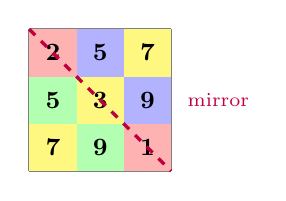
\begin{tikzpicture}[scale=1.0]
    % Matrix grid
    \draw[black!50, thick] (0,0) grid[step=0.6] (1.8,1.8);

    % Fill symmetric entries with same colors
    \fill[red!30] (0,1.2) rectangle (0.6,1.8);
    \fill[red!30] (1.2,0) rectangle (1.8,0.6);

    \fill[blue!30] (0.6,1.2) rectangle (1.2,1.8);
    \fill[blue!30] (1.2,0.6) rectangle (1.8,1.2);

    \fill[green!30] (0,0.6) rectangle (0.6,1.2);
    \fill[green!30] (0.6,0) rectangle (1.2,0.6);

    % Diagonal
    \fill[yellow!50] (0,0) rectangle (0.6,0.6);
    \fill[yellow!50] (0.6,0.6) rectangle (1.2,1.2);
    \fill[yellow!50] (1.2,1.2) rectangle (1.8,1.8);

    % Numbers
    \node[font=\small\bfseries] at (0.3,1.5) {2};
    \node[font=\small\bfseries] at (0.9,1.5) {5};
    \node[font=\small\bfseries] at (1.5,1.5) {7};
    \node[font=\small\bfseries] at (0.3,0.9) {5};
    \node[font=\small\bfseries] at (0.9,0.9) {3};
    \node[font=\small\bfseries] at (1.5,0.9) {9};
    \node[font=\small\bfseries] at (0.3,0.3) {7};
    \node[font=\small\bfseries] at (0.9,0.3) {9};
    \node[font=\small\bfseries] at (1.5,0.3) {1};

    % Diagonal mirror line
    \draw[purple, very thick, dashed] (0,1.8) -- (1.8,0);

    % Label
    \node[purple, font=\scriptsize] at (2.4,0.9) {mirror};
\end{tikzpicture}

\vspace{0.5cm}

$\mat{A} = \begin{bmatrix} 2 & 5 & 7 \\ 5 & 3 & 9 \\ 7 & 9 & 1 \end{bmatrix}$ \quad Mirror property: $a_{ij} = a_{ji}$
\end{center}
\vspace{0.3cm}

\begin{definition}{Symmetric Matrix}{}
A matrix $\mat{A}$ is symmetric if $a_{ij} = a_{ji}$ for all $i, j$.

In other words, it's symmetric across the main diagonal (top-left to bottom-right).
\end{definition}

\begin{example}
\[
\mat{A} = \begin{bmatrix}
1 & 2 & 3 \\
2 & 5 & 6 \\
3 & 6 & 9
\end{bmatrix}
\]

Notice: top-right matches bottom-left (both have 2), etc.
\[
\mat{A}^\top = \begin{bmatrix}
1 & 2 & 3 \\
2 & 5 & 6 \\
3 & 6 & 9
\end{bmatrix} = \mat{A}
\]
\end{example}

\textbf{Why care about symmetric matrices?}
\begin{itemize}
    \item They represent undirected relationships (if A likes B, then B likes A)
    \item They have special mathematical properties (real eigenvalues, orthogonal eigenvectors---we'll learn these later!)
    \item They're easier to work with computationally
\end{itemize}

\begin{intuition}
\textbf{Symmetric Matrices in Real Life}

\textbf{Distance matrices:} The distance from city A to city B equals the distance from B to A. Symmetric!

\textbf{Similarity matrices:} If your taste is similar to mine, mine is similar to yours. Symmetric!

\textbf{Correlation matrices:} The correlation between height and weight equals the correlation between weight and height. Symmetric!

\textbf{Social networks (undirected):} If we're friends, you're my friend and I'm yours. Symmetric! (Directed networks like Twitter followers are NOT symmetric---I might follow you but you might not follow me back. Sad.)
\end{intuition}

\begin{connection}
\textbf{Covariance matrices} (which measure how variables relate to each other) are always symmetric. When training neural networks, we sometimes encounter symmetric matrices in optimization (the Hessian matrix of second derivatives).

\textbf{Fun fact:} Symmetric matrices have a beautiful guarantee---their eigenvectors are always orthogonal (perpendicular to each other). This makes them much easier to decompose and understand. We'll explore this magic in Chapter 2!
\end{connection}

\section{Linear Combinations and Span: Building Blocks of Vector Spaces}

Now for some deeper concepts. Don't worry—we'll keep it intuitive! These ideas are fundamental to understanding how neural networks represent and manipulate information.

\subsection{Linear Combinations: Mixing and Matching}

A \vocab{linear combination} is just adding scaled versions of vectors. It's the fundamental operation for building new vectors from old ones.

\begin{definition}{Linear Combination}{}
Given vectors $\vect{v}_1, \vect{v}_2, \ldots, \vect{v}_k$ and scalars $c_1, c_2, \ldots, c_k$, the linear combination is:
\[
c_1 \vect{v}_1 + c_2 \vect{v}_2 + \cdots + c_k \vect{v}_k
\]
\end{definition}

\begin{intuition}
\textbf{Analogy: The Smoothie Bar}

Imagine a smoothie bar with base ingredients:
\begin{itemize}
    \item Banana smoothie base = $\vect{v}_1$ (creamy, sweet, yellow)
    \item Berry smoothie base = $\vect{v}_2$ (tart, red, antioxidant-rich)
    \item Green smoothie base = $\vect{v}_3$ (healthy, green, earthy)
\end{itemize}

A linear combination is your custom order:
\[
\text{Your drink} = 0.5 \times \text{Banana} + 0.3 \times \text{Berry} + 0.2 \times \text{Green}
\]

The scalars (0.5, 0.3, 0.2) are your "recipe"—how much of each base to use. Different scalars = different smoothies! Every possible smoothie you can make is a linear combination of the bases.

\textbf{The key insight:} With a good set of base ingredients, you can create an enormous variety of outputs. This is exactly how neural networks work—they learn useful "base vectors" and then combine them differently for different inputs!
\end{intuition}

\begin{example}
Let $\vect{v}_1 = [1, 0]$ and $\vect{v}_2 = [0, 1]$. Then:
\[
3\vect{v}_1 + 5\vect{v}_2 = 3\begin{bmatrix} 1 \\ 0 \end{bmatrix} + 5\begin{bmatrix} 0 \\ 1 \end{bmatrix} = \begin{bmatrix} 3 \\ 0 \end{bmatrix} + \begin{bmatrix} 0 \\ 5 \end{bmatrix} = \begin{bmatrix} 3 \\ 5 \end{bmatrix}
\]

We built $[3, 5]$ from $[1, 0]$ and $[0, 1]$!

In fact, ANY 2D vector can be built from $[1, 0]$ and $[0, 1]$:
\[
\begin{bmatrix} x \\ y \end{bmatrix} = x\begin{bmatrix} 1 \\ 0 \end{bmatrix} + y\begin{bmatrix} 0 \\ 1 \end{bmatrix}
\]

These two vectors are the "ultimate bases"—from them, you can create any 2D vector!
\end{example}

\begin{example}
\textbf{Color Mixing as Linear Combinations}

In RGB color space, every color is a linear combination of red, green, and blue:
\[
\text{Purple} = 0.5 \times \text{Red} + 0.0 \times \text{Green} + 0.5 \times \text{Blue}
\]
\[
\text{Yellow} = 1.0 \times \text{Red} + 1.0 \times \text{Green} + 0.0 \times \text{Blue}
\]
\[
\text{White} = 1.0 \times \text{Red} + 1.0 \times \text{Green} + 1.0 \times \text{Blue}
\]

The three primary colors are your "basis vectors," and the scalars (between 0 and 1) determine the exact shade. Every color on your screen right now is a linear combination!
\end{example}

\begin{intuition}
Linear combinations are like recipes. You have ingredients (vectors) and amounts (scalars), and you mix them to create something new.

\textbf{Geometric view:} If you have two arrows in 2D that aren't parallel, you can reach any point in the plane by scaling and adding them. They "span" the entire 2D space.

\begin{center}
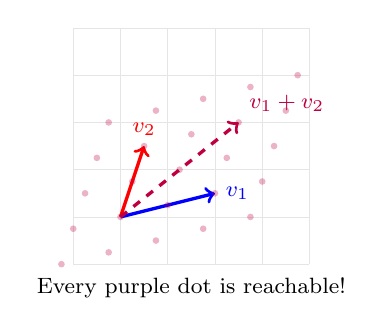
\begin{tikzpicture}[scale=0.6]
    % Grid showing reachable points
    \draw[very thin,gray!20] (-1,-1) grid (4,4);

    % Base vectors
    \draw[->,very thick,blue] (0,0) -- (2,0.5) node[right] {\footnotesize $\vect{v}_1$};
    \draw[->,very thick,red] (0,0) -- (0.5,1.5) node[above] {\footnotesize $\vect{v}_2$};

    % Some example combinations (dots)
    \foreach \a in {-0.5,0,0.5,1,1.5} {
        \foreach \b in {-0.5,0,0.5,1,1.5} {
            \fill[purple,opacity=0.3] ({\a*2+\b*0.5},{\a*0.5+\b*1.5}) circle (2pt);
        }
    }

    % One highlighted combination
    \draw[->,very thick,purple,dashed] (0,0) -- (2.5,2) node[above right] {\footnotesize $\vect{v}_1 + \vect{v}_2$};

    \node at (1.5,-1.5) {\footnotesize Every purple dot is reachable!};
\end{tikzpicture}
\end{center}
\end{intuition}

\subsection{Span: What Can You Reach?}

The \vocab{span} of a set of vectors is all the linear combinations you can make from them. Think of it as your "reachable territory."

\begin{definition}{Span}{}
The span of vectors $\{\vect{v}_1, \vect{v}_2, \ldots, \vect{v}_k\}$ is:
\[
\text{span}(\vect{v}_1, \ldots, \vect{v}_k) = \{c_1\vect{v}_1 + \cdots + c_k\vect{v}_k : c_1, \ldots, c_k \in \R\}
\]

It's the set of all points you can reach by mixing these vectors.
\end{definition}

\begin{intuition}
\textbf{Analogy: The Video Game Map}

Imagine you're in a video game. Your "movement vectors" determine where you can go:

\begin{itemize}
    \item \textbf{One movement vector (e.g., "walk forward"):} You can only move along a line. Your span is 1D!
    \item \textbf{Two independent vectors (e.g., "forward" + "strafe right"):} You can reach any point on the ground. Your span is a 2D plane!
    \item \textbf{Three independent vectors (add "jump/fly"):} You can reach any point in 3D space. Your span is all of 3D!
\end{itemize}

\textbf{The key question:} Given your available movements (vectors), what territory can you explore?

\begin{center}
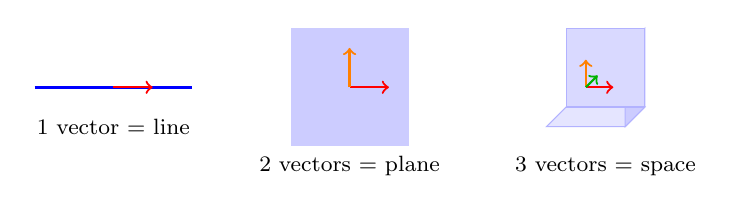
\begin{tikzpicture}[scale=0.5]
    % 1D span
    \begin{scope}
        \draw[very thick,blue] (-2,0) -- (2,0);
        \draw[->,thick,red] (0,0) -- (1,0);
        \node at (0,-1) {\footnotesize 1 vector = line};
    \end{scope}

    % 2D span
    \begin{scope}[xshift=6cm]
        \fill[blue!20] (-1.5,-1.5) rectangle (1.5,1.5);
        \draw[->,thick,red] (0,0) -- (1,0);
        \draw[->,thick,orange] (0,0) -- (0,1);
        \node at (0,-2) {\footnotesize 2 vectors = plane};
    \end{scope}

    % 3D span (represented as cube)
    \begin{scope}[xshift=12cm]
        \draw[blue!30,fill=blue!10] (-1,-1) -- (1,-1) -- (1.5,-0.5) -- (-0.5,-0.5) -- cycle;
        \draw[blue!30,fill=blue!20] (1,-1) -- (1,1) -- (1.5,1.5) -- (1.5,-0.5) -- cycle;
        \draw[blue!30,fill=blue!15] (-0.5,-0.5) -- (1.5,-0.5) -- (1.5,1.5) -- (-0.5,1.5) -- cycle;
        \draw[->,thick,red] (0,0) -- (0.7,0);
        \draw[->,thick,orange] (0,0) -- (0,0.7);
        \draw[->,thick,green!70!black] (0,0) -- (0.3,0.3);
        \node at (0.5,-2) {\footnotesize 3 vectors = space};
    \end{scope}
\end{tikzpicture}
\end{center}
\end{intuition}

\begin{example}
\textbf{1D line:} If $\vect{v} = [1, 2]$, then $\text{span}(\vect{v})$ is all vectors of the form $c[1, 2] = [c, 2c]$. This is a line through the origin!

\textbf{2D plane:} If $\vect{v}_1 = [1, 0, 0]$ and $\vect{v}_2 = [0, 1, 0]$, then $\text{span}(\vect{v}_1, \vect{v}_2)$ is the entire $xy$-plane in 3D space.

\textbf{All of 3D:} If $\vect{v}_1 = [1, 0, 0]$, $\vect{v}_2 = [0, 1, 0]$, $\vect{v}_3 = [0, 0, 1]$, then $\text{span}(\vect{v}_1, \vect{v}_2, \vect{v}_3) = \R^3$ (all of 3D space!)
\end{example}

\begin{intuition}
\textbf{The "Can I Get There?" Test}

Given a target vector $\vect{w}$ and some vectors $\vect{v}_1, \vect{v}_2, \ldots$, asking "Is $\vect{w}$ in the span?" is the same as asking:

"Can I find scalars $c_1, c_2, \ldots$ such that $c_1\vect{v}_1 + c_2\vect{v}_2 + \cdots = \vect{w}$?"

If yes: $\vect{w}$ is in the span. You can reach it!

If no: $\vect{w}$ is outside the span. You're stuck—you can't get there from here.

\textbf{Example:} Can you reach $[3, 5]$ using only $\vect{v} = [1, 2]$?

You need: $c \cdot [1, 2] = [3, 5]$, which means $c = 3$ AND $c = 2.5$. Contradiction! So $[3, 5]$ is NOT in the span of $[1, 2]$. With only one vector, you're trapped on a line, and $[3, 5]$ isn't on that line.
\end{intuition}

\begin{connection}
\textbf{Span in Neural Networks}

When a neural network learns word embeddings, it's essentially learning a set of "basis concepts." The span of these basis concepts determines what the network can represent.

If the embedding dimension is 768 (like in BERT), the network has 768 "direction" it can use. The span of all possible embeddings is a 768-dimensional space. Every word, sentence, or document the model processes lives somewhere in this vast span!

\textbf{The representation bottleneck:} If your basis vectors don't span a rich enough space, some concepts literally cannot be represented. This is why embedding dimension matters—too small, and important distinctions get lost.
\end{connection}

\subsection{Linear Independence: No Redundancy}

Vectors are \vocab{linearly independent} if none of them is a combination of the others. No redundancy!

\begin{definition}{Linear Independence}{}
Vectors $\vect{v}_1, \ldots, \vect{v}_k$ are linearly independent if:
\[
c_1\vect{v}_1 + \cdots + c_k\vect{v}_k = \vect{0} \quad \text{implies} \quad c_1 = \cdots = c_k = 0
\]

In plain English: The only way to combine them to get zero is by using all zero coefficients.
\end{definition}

\begin{example}
\textbf{Independent:} $\vect{v}_1 = [1, 0]$ and $\vect{v}_2 = [0, 1]$ are independent. Neither is a multiple of the other.

\textbf{Dependent:} $\vect{v}_1 = [1, 2]$, $\vect{v}_2 = [2, 4]$, and $\vect{v}_3 = [3, 6]$ are dependent because $\vect{v}_2 = 2\vect{v}_1$ and $\vect{v}_3 = 3\vect{v}_1$. They're all on the same line!

If you have $\vect{v}_1$, you don't need $\vect{v}_2$ or $\vect{v}_3$—they're redundant.
\end{example}

\begin{intuition}
Think of vectors as directions you can move. If they're independent, each one gives you a new direction. If they're dependent, at least one is a combo of the others—it doesn't give you anything new.

In 2D, you can have at most 2 independent vectors (like north-south and east-west). In 3D, at most 3 (add up-down). In $n$ dimensions, at most $n$.
\end{intuition}

\begin{intuition}
\textbf{Analogy: The Band Member Test}

Imagine you're forming a band:
\begin{itemize}
    \item \textbf{Guitarist, drummer, singer} = Independent! Each brings something unique.
    \item \textbf{Guitarist, another guitarist who plays the exact same notes} = Dependent! One is redundant.
    \item \textbf{Guitarist, bassist who always plays the guitar part but lower} = Dependent! The bassist doesn't add new information---they're just a scaled version of the guitarist.
\end{itemize}

\textbf{The Dimension Game:}

Here's a fun way to check independence: Can you "fake" any vector using the others?

\begin{center}
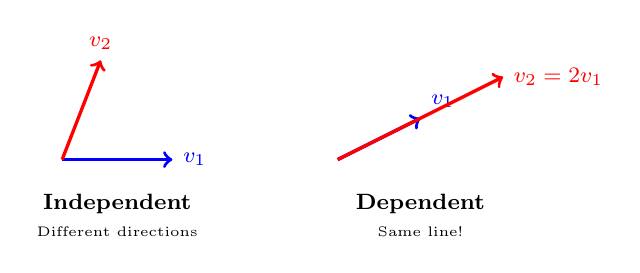
\begin{tikzpicture}[scale=0.7]
    % Independent case
    \begin{scope}
        \draw[->,very thick,blue] (0,0) -- (2,0) node[right] {\footnotesize $\vect{v}_1$};
        \draw[->,very thick,red] (0,0) -- (0.7,1.8) node[above] {\footnotesize $\vect{v}_2$};
        \node at (1,-0.8) {\footnotesize \textbf{Independent}};
        \node at (1,-1.3) {\tiny Different directions};
    \end{scope}

    % Dependent case
    \begin{scope}[xshift=5cm]
        \draw[->,very thick,blue] (0,0) -- (1.5,0.75) node[above right] {\footnotesize $\vect{v}_1$};
        \draw[->,very thick,red] (0,0) -- (3,1.5) node[right] {\footnotesize $\vect{v}_2 = 2\vect{v}_1$};
        \node at (1.5,-0.8) {\footnotesize \textbf{Dependent}};
        \node at (1.5,-1.3) {\tiny Same line!};
    \end{scope}
\end{tikzpicture}
\end{center}

If all your vectors lie on a line (in 2D) or a plane (in 3D), they're dependent. You need vectors that "escape" into new dimensions!
\end{intuition}

\begin{connection}
\textbf{Why this matters for LLMs:}

Word embeddings should ideally be "efficient"—each dimension should capture something unique. If dimension 47 and dimension 892 always move together (they're dependent), you're wasting space.

Good training procedures tend to produce embeddings where dimensions are mostly independent, capturing different aspects of meaning.
\end{connection}

\section{Rank: The True Dimension of a Matrix}

The \vocab{rank} of a matrix tells you how many truly independent rows (or columns) it has.

\begin{definition}{Matrix Rank}{}
The rank of matrix $\mat{A}$ is the maximum number of linearly independent columns (or equivalently, rows).

It's the "dimensionality" of the output space when you multiply by $\mat{A}$.
\end{definition}

\begin{example}
\[
\mat{A} = \begin{bmatrix}
1 & 2 \\
2 & 4
\end{bmatrix}
\]

Row 2 is 2 times row 1, so they're dependent. Rank = 1.

\[
\mat{B} = \begin{bmatrix}
1 & 0 \\
0 & 1
\end{bmatrix}
\]

Both rows are independent. Rank = 2 (full rank!).
\end{example}

\begin{intuition}
Rank tells you: "How many independent directions does this matrix output?"

A rank-1 matrix squashes everything onto a line. A rank-2 matrix (in 3D) squashes onto a plane. A full-rank $n \times n$ matrix doesn't squash at all—it just rotates/scales space.
\end{intuition}

\begin{intuition}
\textbf{Analogy: The Information Funnel}

Think of matrix rank as how much a funnel narrows:

\begin{center}
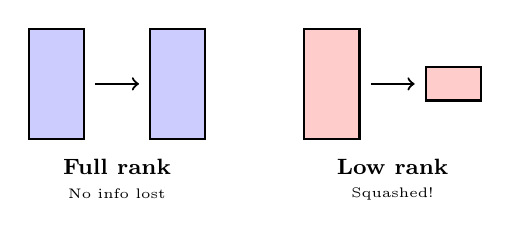
\begin{tikzpicture}[scale=0.7]
    % Full rank (no narrowing)
    \begin{scope}
        \draw[thick,fill=blue!20] (0,2) -- (1,2) -- (1,0) -- (0,0) -- cycle;
        \draw[->,thick] (1.2,1) -- (2,1);
        \draw[thick,fill=blue!20] (2.2,2) -- (3.2,2) -- (3.2,0) -- (2.2,0) -- cycle;
        \node at (1.6,-0.5) {\footnotesize \textbf{Full rank}};
        \node at (1.6,-1) {\tiny No info lost};
    \end{scope}

    % Rank deficient (narrowing)
    \begin{scope}[xshift=5cm]
        \draw[thick,fill=red!20] (0,2) -- (1,2) -- (1,0) -- (0,0) -- cycle;
        \draw[->,thick] (1.2,1) -- (2,1);
        \draw[thick,fill=red!20] (2.2,1.3) -- (3.2,1.3) -- (3.2,0.7) -- (2.2,0.7) -- cycle;
        \node at (1.6,-0.5) {\footnotesize \textbf{Low rank}};
        \node at (1.6,-1) {\tiny Squashed!};
    \end{scope}
\end{tikzpicture}
\end{center}

\begin{itemize}
    \item \textbf{Rank = n (full):} All information preserved. You could reverse the transformation.
    \item \textbf{Rank = n-1:} One dimension squashed. Like projecting 3D onto a 2D plane.
    \item \textbf{Rank = 1:} Everything collapses to a line. Massive information loss!
    \item \textbf{Rank = 0:} Everything becomes zero. Total annihilation of information.
\end{itemize}
\end{intuition}

\begin{example}
\textbf{Visualizing Rank Deficiency}

Consider these two $3 \times 3$ matrices and what they do to a cube:

\textbf{Full rank (rank = 3):}
\[
\mat{A} = \begin{bmatrix}
1 & 0 & 0 \\
0 & 1 & 0 \\
0 & 0 & 1
\end{bmatrix}
\]
The cube stays a cube. All 3 dimensions preserved.

\textbf{Rank = 2:}
\[
\mat{B} = \begin{bmatrix}
1 & 0 & 0 \\
0 & 1 & 0 \\
0 & 0 & 0
\end{bmatrix}
\]
The cube becomes a flat square! The z-dimension is gone---squashed to zero.

\textbf{Rank = 1:}
\[
\mat{C} = \begin{bmatrix}
1 & 0 & 0 \\
0 & 0 & 0 \\
0 & 0 & 0
\end{bmatrix}
\]
The cube becomes a line! Only the x-dimension survives.
\end{example}

\begin{connection}
\textbf{Low-rank matrices in deep learning:}

It turns out many weight matrices in neural networks are approximately low-rank. This is the basis for techniques like Low-Rank Adaptation (LoRA), which fine-tunes LLMs efficiently by only updating low-rank components of weight matrices!

\textbf{Why are neural network weights often low-rank?}

This is still being researched, but some theories:
\begin{itemize}
    \item The network learns to focus on a few important "directions" in the data
    \item Regularization pushes weights toward simpler (lower-rank) solutions
    \item The actual structure in language/images is lower-dimensional than the embedding space
\end{itemize}

LoRA exploits this by saying: "Instead of updating a huge $d \times d$ matrix, let's just update a small $d \times r$ and $r \times d$ pair, where $r \ll d$." This can reduce trainable parameters by 10,000x while maintaining performance!
\end{connection}

\section{Matrix Inverse: The Undo Button}

The \vocab{inverse} of a matrix "undoes" what the matrix does.

\begin{definition}{Matrix Inverse}{}
For a square matrix $\mat{A}$, if there exists a matrix $\mat{A}^{-1}$ such that:
\[
\mat{A}\mat{A}^{-1} = \mat{A}^{-1}\mat{A} = \mat{I}
\]

then $\mat{A}^{-1}$ is the inverse of $\mat{A}$.

Not all matrices have inverses! Only square, full-rank matrices do.
\end{definition}

\begin{example}
\[
\mat{A} = \begin{bmatrix}
1 & 2 \\
3 & 4
\end{bmatrix}
\quad
\mat{A}^{-1} = \begin{bmatrix}
-2 & 1 \\
1.5 & -0.5
\end{bmatrix}
\]

Check:
\[
\mat{A}\mat{A}^{-1} = \begin{bmatrix}
1 & 2 \\
3 & 4
\end{bmatrix}
\begin{bmatrix}
-2 & 1 \\
1.5 & -0.5
\end{bmatrix}
= \begin{bmatrix}
1 & 0 \\
0 & 1
\end{bmatrix} = \mat{I}
\]
\end{example}

\begin{intuition}
If multiplying by $\mat{A}$ is like putting on a pair of glasses that distorts your vision, multiplying by $\mat{A}^{-1}$ takes the glasses off and returns you to normal.
\end{intuition}

\subsection{When Does an Inverse NOT Exist? (The Fun Part!)}

Not every matrix has an inverse. This isn't just a mathematical technicality---it's actually a profound statement about \textit{information loss}. Let's explore the different ways a matrix can be "non-invertible" (also called \vocab{singular}).

\begin{intuition}
\textbf{The Core Idea: You Can't Unscramble an Egg}

A matrix inverse only exists when you can perfectly reverse whatever the matrix did. If the matrix \textit{destroys information} in any way, there's no going back. It's like trying to:
\begin{itemize}
    \item Unblend a smoothie back into strawberries and bananas
    \item Figure out exactly what someone said from just hearing "mmhmm" on the phone
    \item Recover a deleted file after the hard drive has been overwritten
\end{itemize}

Once information is gone, it's \textit{gone}.
\end{intuition}

\subsubsection{Reason 1: The Matrix Isn't Square}

\textbf{The Rule:} Only square matrices (same number of rows and columns) can have inverses.

\textbf{Why?} Think about what a non-square matrix does:

\begin{itemize}
    \item A $3 \times 2$ matrix takes 2D vectors and outputs 3D vectors
    \item A $2 \times 3$ matrix takes 3D vectors and outputs 2D vectors
\end{itemize}

\begin{example}
Consider a $2 \times 3$ matrix that goes from 3D to 2D:
\[
\mat{A} = \begin{bmatrix}
1 & 0 & 0 \\
0 & 1 & 0
\end{bmatrix}
\]

This matrix takes a 3D point and "forgets" the z-coordinate:
\[
\begin{bmatrix}
1 & 0 & 0 \\
0 & 1 & 0
\end{bmatrix}
\begin{bmatrix}
x \\ y \\ z
\end{bmatrix}
= \begin{bmatrix}
x \\ y
\end{bmatrix}
\]

The z-value is completely lost! If I give you the output $[3, 5]$, you can't tell me if the original was $[3, 5, 0]$ or $[3, 5, 1000]$ or $[3, 5, -42]$. Infinitely many 3D points map to the same 2D point.

\textbf{No inverse can exist} because there's no unique answer to "undo."
\end{example}

\begin{intuition}
\textbf{Analogy: The Shadow Projector}

Imagine shining a flashlight on a 3D object and looking at its 2D shadow on the wall. Many different 3D objects can cast the \textit{exact same shadow}. A tall thin cylinder and a sphere might both cast circular shadows.

Going from 3D object $\rightarrow$ 2D shadow is a non-square transformation. You can't "un-project" a shadow back to the original 3D object because you've lost the depth information!
\end{intuition}

\subsubsection{Reason 2: The Matrix Squashes a Dimension (Determinant = 0)}

Even square matrices can fail to have inverses! This happens when the matrix \vocab{collapses} or \vocab{squashes} space.

\begin{definition}{Singular Matrix}{}
A square matrix with no inverse is called \textbf{singular} or \textbf{degenerate}. This happens when its determinant equals zero: $\det(\mat{A}) = 0$.
\end{definition}

\begin{example}
Consider this sneaky matrix:
\[
\mat{A} = \begin{bmatrix}
1 & 2 \\
2 & 4
\end{bmatrix}
\]

Notice that the second row is just $2\times$ the first row! Let's see what this matrix does to some vectors:
\begin{align*}
\begin{bmatrix}
1 & 2 \\
2 & 4
\end{bmatrix}
\begin{bmatrix}
1 \\ 0
\end{bmatrix}
&= \begin{bmatrix}
1 \\ 2
\end{bmatrix} \\[0.5em]
\begin{bmatrix}
1 & 2 \\
2 & 4
\end{bmatrix}
\begin{bmatrix}
0 \\ 1
\end{bmatrix}
&= \begin{bmatrix}
2 \\ 4
\end{bmatrix}
\end{align*}

Both outputs point in the same direction! This matrix squashes all of 2D space down onto a single line.
\end{example}

\begin{intuition}
\textbf{Analogy: The Pancake Press}

Imagine a 3D cube of dough. A singular matrix is like a giant press that squashes the cube completely flat into a 2D pancake.

\begin{center}
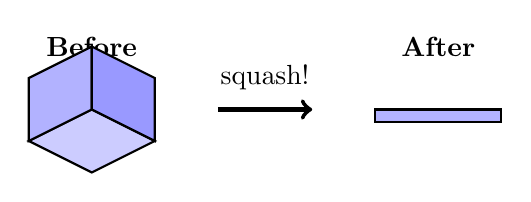
\begin{tikzpicture}[scale=0.8]
    % 3D cube (before)
    \node at (-2, 1.5) {\textbf{Before}};
    \draw[thick, fill=blue!20] (-3,0) -- (-2,0.5) -- (-1,0) -- (-2,-0.5) -- cycle;
    \draw[thick, fill=blue!30] (-3,0) -- (-3,1) -- (-2,1.5) -- (-2,0.5) -- cycle;
    \draw[thick, fill=blue!40] (-2,0.5) -- (-2,1.5) -- (-1,1) -- (-1,0) -- cycle;

    % Arrow
    \draw[->, ultra thick] (0,0.5) -- (1.5,0.5);
    \node at (0.75, 1) {squash!};

    % Flat pancake (after)
    \node at (3.5, 1.5) {\textbf{After}};
    \draw[thick, fill=blue!30] (2.5,0.3) -- (4.5,0.3) -- (4.5,0.5) -- (2.5,0.5) -- cycle;
\end{tikzpicture}
\end{center}

Once it's flat, you've lost the height information forever. Was the original cube 1 inch tall? 10 inches? 100 inches? The pancake can't tell you. \textbf{You can't un-squash a pancake back into a cube.}
\end{intuition}

\subsubsection{Reason 3: Multiple Inputs Give the Same Output}

This is really the same as Reason 2, but it's worth seeing from another angle.

\begin{example}
Using that same singular matrix:
\[
\mat{A} = \begin{bmatrix}
1 & 2 \\
2 & 4
\end{bmatrix}
\]

Watch what happens to these two \textit{different} inputs:
\[
\mat{A} \begin{bmatrix}
4 \\ 1
\end{bmatrix}
= \begin{bmatrix}
6 \\ 12
\end{bmatrix}
\quad \text{and} \quad
\mat{A} \begin{bmatrix}
2 \\ 2
\end{bmatrix}
= \begin{bmatrix}
6 \\ 12
\end{bmatrix}
\]

Two completely different inputs produce the \textit{exact same output}!

If an inverse existed and you asked it "What input gives $[6, 12]$?" it would have to answer both $[4, 1]$ AND $[2, 2]$. But a function can only give one answer. Contradiction! So no inverse can exist.
\end{example}

\begin{intuition}
\textbf{Analogy: The Hash Function Problem}

This is exactly why cryptographic hash functions (like SHA-256) have no inverse. Many different passwords hash to... wait, actually good hash functions are designed so collisions are astronomically rare.

Better analogy: It's like a "round to nearest integer" function. Both $3.2$ and $3.7$ round to $4$. If I tell you the answer is $4$, you can't know what the original number was. The rounding function has no inverse!
\end{intuition}

\subsubsection{The Determinant: Your Singularity Detector}

The \vocab{determinant} is a single number that tells you whether a matrix is invertible:

\begin{itemize}
    \item $\det(\mat{A}) \neq 0$ $\Rightarrow$ Inverse exists! Matrix is \textbf{invertible/non-singular}
    \item $\det(\mat{A}) = 0$ $\Rightarrow$ No inverse. Matrix is \textbf{singular}
\end{itemize}

For a $2 \times 2$ matrix $\begin{bmatrix} a & b \\ c & d \end{bmatrix}$, the determinant is:
\[
\det = ad - bc
\]

\begin{example}
\textbf{Invertible matrix:}
\[
\mat{A} = \begin{bmatrix}
1 & 2 \\
3 & 4
\end{bmatrix}
\quad \Rightarrow \quad \det(\mat{A}) = (1)(4) - (2)(3) = 4 - 6 = -2 \neq 0 \quad \checkmark
\]

\textbf{Singular matrix:}
\[
\mat{B} = \begin{bmatrix}
1 & 2 \\
2 & 4
\end{bmatrix}
\quad \Rightarrow \quad \det(\mat{B}) = (1)(4) - (2)(2) = 4 - 4 = 0 \quad \text{(no inverse!)}
\]
\end{example}

\begin{intuition}
\textbf{What Does the Determinant Measure?}

Geometrically, the determinant measures how much a matrix \textbf{scales area} (in 2D) or \textbf{volume} (in 3D).

\begin{itemize}
    \item $|\det| = 2$ means areas get doubled
    \item $|\det| = 0.5$ means areas get halved
    \item $|\det| = 0$ means areas get squashed to zero (a line or a point)
    \item Negative determinant means the transformation also flips/mirrors space
\end{itemize}

A determinant of zero means the matrix squashes all of space down to a lower dimension---and you can't stretch a line back into a full 2D plane!
\end{intuition}

\subsubsection{Summary: The Three Strikes of Non-Invertibility}

A matrix has NO inverse if any of these are true:

\begin{enumerate}
    \item \textbf{Not square:} Going between different dimensions loses information
    \item \textbf{Determinant is zero:} The matrix squashes space (rows/columns are linearly dependent)
    \item \textbf{Not full rank:} Equivalent to \#2---some dimensions get collapsed
\end{enumerate}

\begin{connection}
\textbf{Why This Matters for Machine Learning:}

When training neural networks, we often need to solve equations like $\mat{A}\vect{x} = \vect{b}$. If $\mat{A}$ is invertible, the answer is simply $\vect{x} = \mat{A}^{-1}\vect{b}$. Easy!

But if $\mat{A}$ is singular (or nearly singular---called \vocab{ill-conditioned}), we're in trouble:
\begin{itemize}
    \item The equation might have \textit{no solution} (the $\vect{b}$ we want isn't reachable)
    \item The equation might have \textit{infinitely many solutions} (we squashed dimensions, so many inputs work)
    \item Numerically, even "almost singular" matrices cause wild instability
\end{itemize}

This is why techniques like \textbf{regularization} (adding small values to the diagonal) and \textbf{pseudoinverses} are so important in ML---they help us handle these degenerate cases gracefully!
\end{connection}

\begin{connection}
\textbf{In machine learning:}

Matrix inverses show up in:
\begin{itemize}
    \item Solving systems of equations (finding optimal weights)
    \item Computing certain derivatives
    \item Some optimization algorithms (Newton's method)
\end{itemize}

However, computing inverses is expensive and numerically unstable, so we often use tricks to avoid them (like using transposes or pseudoinverses).
\end{connection}

\section{Practice Problems: Time to Get Your Hands Dirty!}

\begin{intuition}
\textbf{Why Practice Matters}

Reading about linear algebra is like reading about swimming. You understand the concepts, but you won't actually \textit{get it} until you do it yourself. These problems are designed to build intuition, not just test memorization.

\textbf{Pro tip:} Don't just compute the answers---think about what they \textit{mean}. When you get a dot product of 150, ask yourself: "Is that big? What does it tell me?" When a matrix transforms a vector, visualize what happened geometrically.
\end{intuition}

\subsection{Problem 1: Vector Operations (The Fundamentals)}

Given $\vect{a} = [2, -1, 3]$ and $\vect{b} = [1, 4, -2]$:

\begin{enumerate}
    \item Compute $\vect{a} + \vect{b}$
    \item Compute $3\vect{a} - 2\vect{b}$
    \item Compute $\vect{a} \cdot \vect{b}$ (Hint: What does the sign tell you about their relationship?)
    \item Compute $\norm{\vect{a}}$
    \item Normalize $\vect{a}$ to get a unit vector $\hat{\vect{a}}$, then verify $\norm{\hat{\vect{a}}} = 1$
\end{enumerate}

\textbf{Bonus challenge:} Are $\vect{a}$ and $\vect{b}$ more "similar" or "different"? How can you tell from the dot product?

\subsection{Problem 2: Matrix Multiplication (Transformations in Action)}

Given:
\[
\mat{A} = \begin{bmatrix}
1 & 2 \\
3 & 4
\end{bmatrix}, \quad
\vect{x} = \begin{bmatrix}
5 \\
6
\end{bmatrix}, \quad
\mat{B} = \begin{bmatrix}
2 & 0 \\
1 & 3
\end{bmatrix}
\]

\begin{enumerate}
    \item Compute $\mat{A}\vect{x}$ (Where does $\vect{x}$ go?)
    \item Compute $\mat{A}\mat{B}$ (Composing two transformations)
    \item Compute $\mat{B}\mat{A}$ (Is it different from $\mat{A}\mat{B}$?)
    \item Compute $\mat{A}^\top$ (Flip rows and columns)
    \item \textbf{Challenge:} What is $\det(\mat{A})$? Is $\mat{A}$ invertible?
\end{enumerate}

\subsection{Problem 3: The Dating App Similarity Challenge}

Imagine a dating app where users rate their preferences on a 1-10 scale:

\begin{center}
\begin{tabular}{lccccc}
\textbf{Person} & \textbf{Outdoors} & \textbf{Reading} & \textbf{Gaming} & \textbf{Cooking} & \textbf{Travel} \\
\hline
You & 8 & 6 & 9 & 4 & 7 \\
Alex & 9 & 5 & 10 & 3 & 8 \\
Jordan & 3 & 9 & 2 & 8 & 4 \\
Sam & 7 & 7 & 7 & 7 & 7 \\
\end{tabular}
\end{center}

\begin{enumerate}
    \item Compute the dot product between You and each other person
    \item Who is most compatible with You? (Highest dot product)
    \item Who is least compatible?
    \item \textbf{Thinking deeper:} Sam rated everything 7. What's special about Sam's compatibility score with everyone? Why?
    \item \textbf{Challenge:} If you normalized everyone's vectors first (made them length 1), would the compatibility rankings change? Why might this be fairer?
\end{enumerate}

\subsection{Problem 4: Thinking About LLMs}

These don't have single "right answers"---they're designed to build intuition:

\begin{enumerate}
    \item If "king" and "queen" have a high dot product, what does that suggest about how the model views these words?

    \item If "king" and "banana" have a dot product close to zero, what does that mean?

    \item GPT-4 has 12,288-dimensional embeddings and a vocabulary of ~100,000 tokens. If you wanted to find the most similar word to "happy," you'd compute 100,000 dot products. Each dot product requires 12,288 multiplications and additions. Roughly how many arithmetic operations is that? (No calculator needed---just estimate the order of magnitude!)

    \item Why do you think AI researchers chose such high dimensions (12,288) instead of, say, 100? What's the trade-off?

    \item \textbf{Brain teaser:} If $\text{king} - \text{man} + \text{woman} \approx \text{queen}$, what might $\text{Paris} - \text{France} + \text{Japan}$ equal? Why?
\end{enumerate}

\subsection{Problem 5: Linear Independence (Spotting Redundancy)}

For each set of vectors, determine: Are they linearly independent? What's their span?

\textbf{Set A:}
\[
\vect{v}_1 = \begin{bmatrix} 1 \\ 2 \\ 3 \end{bmatrix}, \quad
\vect{v}_2 = \begin{bmatrix} 2 \\ 4 \\ 6 \end{bmatrix}, \quad
\vect{v}_3 = \begin{bmatrix} 1 \\ 0 \\ 1 \end{bmatrix}
\]

\textbf{Set B:}
\[
\vect{u}_1 = \begin{bmatrix} 1 \\ 0 \\ 0 \end{bmatrix}, \quad
\vect{u}_2 = \begin{bmatrix} 0 \\ 1 \\ 0 \end{bmatrix}, \quad
\vect{u}_3 = \begin{bmatrix} 0 \\ 0 \\ 1 \end{bmatrix}
\]

\textbf{Set C:}
\[
\vect{w}_1 = \begin{bmatrix} 1 \\ 1 \end{bmatrix}, \quad
\vect{w}_2 = \begin{bmatrix} 2 \\ 2 \end{bmatrix}, \quad
\vect{w}_3 = \begin{bmatrix} 3 \\ 3 \end{bmatrix}
\]

\textbf{Questions:}
\begin{enumerate}
    \item Which sets are linearly independent?
    \item For the dependent sets, which vector(s) are "redundant"?
    \item What's the dimension of the span for each set?
    \item \textbf{Intuition check:} In Set C, all three vectors lie on a \_\_\_\_ (line/plane/all of 2D space)?
\end{enumerate}

\subsection{Problem 6: The Matrix Detective (Understanding Transformations)}

Without computing, predict what each matrix does to the unit square. Then verify with one test vector!

\textbf{Matrix 1:}
$\mat{A} = \begin{bmatrix} 2 & 0 \\ 0 & 2 \end{bmatrix}$

\textbf{Matrix 2:}
$\mat{B} = \begin{bmatrix} 1 & 0 \\ 0 & -1 \end{bmatrix}$

\textbf{Matrix 3:}
$\mat{C} = \begin{bmatrix} 0 & 1 \\ 1 & 0 \end{bmatrix}$

\textbf{Matrix 4:}
$\mat{D} = \begin{bmatrix} 1 & 0 \\ 0 & 0 \end{bmatrix}$

\textbf{For each matrix, answer:}
\begin{enumerate}
    \item What transformation is it? (Scale? Flip? Rotate? Project? Something else?)
    \item What's the determinant? (Hint: for 2×2, it's $ad - bc$)
    \item Is the matrix invertible?
    \item Apply it to $\vect{v} = [1, 1]^\top$ and verify your prediction
\end{enumerate}

\section{Key Takeaways: What You've Learned}

Congratulations! You've just learned the secret language of AI. Let's recap:

\begin{center}
\textbf{\large The Linear Algebra Cheat Sheet}

\vspace{0.5cm}

\begin{tabular}{|p{5.5cm}|p{5.5cm}|}
\hline
\cellcolor{blue!10}\textbf{Vectors} \newline
Lists of numbers \newline
Represent anything!
&
\cellcolor{green!10}\textbf{Dot Product} \newline
Measures similarity \newline
${>}0$: similar, ${=}0$: unrelated
\\
\hline
\cellcolor{red!10}\textbf{Matrices} \newline
Transformations \newline
Rotate, scale, project
&
\cellcolor{orange!10}\textbf{Inverse} \newline
Undo button \newline
Only if $\det \neq 0$
\\
\hline
\cellcolor{purple!10}\textbf{Rank} \newline
True dimensionality \newline
Info preserved or lost
&
\cellcolor{yellow!20}\textbf{Independence} \newline
No redundancy \newline
Each vector = new info
\\
\hline
\end{tabular}
\end{center}

\begin{enumerate}
    \item \textbf{Vectors are lists of numbers} that represent everything from words to images to preferences. In AI, everything becomes a vector.

    \item \textbf{The dot product measures similarity}—it's the most important operation in modern AI. Positive = similar, zero = unrelated, negative = opposite.

    \item \textbf{Matrices are transformations}—they reshape, rotate, scale, and project vectors. They're the "verbs" of linear algebra.

    \item \textbf{Matrix multiplication is composition}—applying transformations in sequence. Order matters!

    \item \textbf{Linear independence means no redundancy}—each vector/dimension adds something genuinely new.

    \item \textbf{Rank tells you the true dimensionality}—how much information is really there vs. how much was lost.

    \item \textbf{Inverses undo transformations}—but only when no information was lost (full rank, non-zero determinant).

    \item \textbf{Every neural network is just matrix multiplications} (plus some nonlinear functions). That's the whole secret!
\end{enumerate}

\begin{connection}
\textbf{The Punchline: How ChatGPT Actually Works}

When ChatGPT reads "The cat sat on the mat," here's what happens:
\begin{enumerate}
    \item \textbf{Embedding:} Each word becomes a vector (lookup in an embedding table---just a big matrix!)
    \item \textbf{Attention:} Dot products compute which words relate to which (``cat'' attends to ``sat'')
    \item \textbf{Transformation:} Vectors get multiplied by weight matrices (transformed through layers)
    \item \textbf{More attention, more transformations:} Repeat 96 times (in GPT-4)
    \item \textbf{Output:} A probability distribution over next words (more vectors!)
\end{enumerate}

Every single step is linear algebra. Billions of dot products. Trillions of matrix multiplications. That's it. That's the whole secret.

\textbf{You now understand the fundamental language of artificial intelligence.}
\end{connection}

\begin{intuition}
\textbf{What's Next?}

In Chapter 2, we'll go deeper into the structure of matrices:
\begin{itemize}
    \item \textbf{Eigenvectors and eigenvalues:} The "natural directions" of a transformation
    \item \textbf{Eigendecomposition:} Breaking matrices into their fundamental components
    \item \textbf{Singular Value Decomposition (SVD):} The most important decomposition in data science
\end{itemize}

These tools reveal the hidden structure inside matrices---and they're the foundation for understanding how neural networks actually learn what they learn.
\end{intuition}

\vspace{1cm}

\begin{center}
\large\textbf{Ready for Chapter 2? Let's unlock the hidden structure of transformations!}

\vspace{0.5cm}

\textit{``I understood matrices before, but now I \textbf{see} them.''} --- Future you, after Chapter 2
\end{center}
